\documentclass[12pt, a4paper]{report}
\usepackage[utf8]{inputenc}
\usepackage{titlesec}
\titleformat{\chapter}[display]
    {\normalfont\huge\bfseries}
    {} 
    {0pt}
    {\Huge Capitolo~\thechapter: }

\titlespacing*{\chapter}{0pt}{50pt}{40pt}

\newcommand{\preamble}{
    \usepackage[italian]{babel}
    \usepackage{geometry}
    \usepackage{amsmath}
    \usepackage{amssymb}
    \usepackage{graphicx}
    \usepackage{ulem}
    \usepackage{amsthm}
    \usepackage{listings}
    \usepackage{xparse}
    \usepackage{expl3}
    \usepackage{tikz}
    \usepackage[colorlinks=true, linkcolor=blue]{hyperref}
    \usetikzlibrary{calc}
    \let\olditemize\itemize
    \renewcommand\itemize{\olditemize\setlength\itemsep{0em}}
    \geometry{a4paper, left=1cm, right=1cm, top=1cm, bottom=2cm}
    \usepackage[most]{tcolorbox}
    \usepackage{xcolor}

    \newtcbtheorem[auto counter,number within=section]{definitionbox}{Definizione}{
        colback=blue!5!white,
        colframe=blue!75!black,
        fonttitle=\bfseries,
        boxsep=5pt,
        arc=5pt,
        boxrule=1pt,
        title={Definizione}
    }{def}

    \newtcbtheorem[auto counter,number within=section]{theorembox}{Teorema}{
        colback=red!5!white,
        colframe=red!75!black,
        fonttitle=\bfseries,
        boxsep=5pt,
        arc=5pt,
        boxrule=1pt,
        title={Teorema}
    }{thm}

    \newtcbtheorem[auto counter,number within=section]{lemma}{Lemma}{
        colback=red!5!white,
        colframe=red!75!black,
        fonttitle=\bfseries,
        boxsep=5pt,
        arc=5pt,
        boxrule=1pt,
        title={Lemma}
    }{lem}
    
    \tcbset{
        demonstration/.style={
            colback=magenta!5!white, 
            colframe=magenta!75!black,
            boxsep=5pt,
            arc=5pt,
            boxrule=1pt,
            title={\textbf{Dimostrazione}}
        }
    }
    
    \newenvironment{demonstration}[1][]{
        \begin{tcolorbox}[demonstration, ##1]
    }{
        \end{tcolorbox}
    }

    \tcbset{
        exercise/.style={
            colback=orange!5!white, 
            colframe=orange!75!black,
            boxsep=5pt,
            arc=5pt,
            boxrule=1pt,
            title={\textbf{Esercizio}}
        }
    }
    
    \newenvironment{exercise}[1][]{
        \begin{tcolorbox}[exercise, ##1]
    }{
        \end{tcolorbox}
    }

    \tcbset{
        example/.style={
            colback=gray!5!white, 
            colframe=gray!75!black,
            boxsep=5pt,
            arc=5pt,
            boxrule=1pt,
            title={\textbf{Esempio}}
        }
    }
    
    \newenvironment{example}[1][]{
        \begin{tcolorbox}[example, ##1]
    }{
        \end{tcolorbox}
    }

        \tcbset{
        algorithm/.style={
            colback=yellow!5!white, 
            colframe=yellow!75!black,
            boxsep=5pt,
            arc=5pt,
            boxrule=1pt,
            title={\textbf{Algoritmo}}
        }
    }
    
    \newenvironment{algorithm}[1][]{
        \begin{tcolorbox}[algorithm, ##1]
    }{
        \end{tcolorbox}
    }

    \definecolor{codegreen}{rgb}{0,0.6,0}
    \definecolor{codegray}{rgb}{0.5,0.5,0.5}
    \definecolor{codepurple}{rgb}{0.58,0,0.82}
    \definecolor{backcolour}{rgb}{0.95,0.95,0.92}

    \lstdefinestyle{mystyle}{  
        commentstyle=\color{codegreen},
        keywordstyle=\color{magenta},
        numberstyle=\tiny\color{codegray},
        stringstyle=\color{codepurple},
        basicstyle=\ttfamily\footnotesize,
        breakatwhitespace=false,         
        breaklines=true,                 
        captionpos=b,                    
        keepspaces=true,                   
        numbersep=5pt,                  
        showspaces=false,                
        showstringspaces=false,
        showtabs=false,                  
        tabsize=2
    }

    \lstset{style=mystyle}
}

\newcommand{\equivalenceclass}[1]{
    \left[#1\right]_\sim
}

\newcommand{\quotientof}[1]{
    #1/_\sim
}
\newcommand{\imagePath}{Images/logoUni.png}

\newcommand{\customTitlePage}[5]{
    \newcommand{\courseTitle}{#1}
    \newcommand{\authorName}{#2}
    \newcommand{\academicYear}{#3}
    \newcommand{\universityName}{#4}
    
    \begin{titlepage}
        \centering
        \includegraphics[width=0.5\textwidth]{\imagePath}\par\vspace{1cm}
        {\scshape\LARGE \universityName \par}
        \vspace{1.5cm}
        {\huge\bfseries \courseTitle \par}
        \vspace{2cm}
        {\Large\itshape \authorName \par}
        \vfill
        \academicYear
    \end{titlepage}
}

\preamble
\begin{document}
    \customTitlePage{Teoria degli Automi e Calcolabilità}{Lorenzo Vaccarecci}{Anno Accademico 2024/2025}{Università degli Studi di Genova}
    \newpage
    \tableofcontents
    \chapter{Preliminari}
        \section{Alfabeti, stringhe, linguaggi}
            \begin{definitionbox}{Alfabeto}{}
                Insieme finito \textbf{non vuoto} di oggetti detti \textit{simboli}.
            \end{definitionbox}
            \begin{definitionbox}{Stringa}{}
                Una stringa $u$ su un alfabeto $\Sigma$ è una funzione totale da $[1,n]$ in $\Sigma$, per qualche $n\in\mathbb{N}$. 
                $n$ si dice \textit{lunghezza} di $u$ e si indica con $|u|$. 
            \end{definitionbox}
            \begin{itemize}
                \item $[1,n]\rightarrow$ sono le posizioni dei simboli all'interno della stringa 
                \item Per \textbf{funzione totale} intendiamo che per ogni posizione nell'intervallo $[1,n]$ deve avere un simbolo corrispondente 
            \end{itemize}
            Da ora in poi: 
            \begin{itemize}
                \item $\sigma\rightarrow$ simboli generici 
                \item $u,v,w\rightarrow$ stringhe generiche 
                \item $\bigwedge\text{ o }\varepsilon\rightarrow$ stringa vuota con lunghezza zero ($\left|\bigwedge\right|=0$ o $\left|\varepsilon\right|=0$) 
            \end{itemize}
            \begin{definitionbox}{Linguaggio $L$}{}
                E' un insieme di stringhe su $\Sigma$, ossia un sottoinsieme di $\Sigma^*$ \textbf{infinito e numerabile}. 
            \end{definitionbox}
            \begin{itemize}
                \item \textbf{Infinito}: contiene un numero illimitato di elementi 
                \item \textbf{Numerabile}: esiste una funzione iniettiva da $\Sigma^*$ all'insieme dei numeri naturali $\mathbb{N}$ 
            \end{itemize}
            L'insieme $\emptyset$ è un linguaggio che non contiene alcun elemento (neanche la stringa vuota). 
            L'insieme $\{\varepsilon\}$ è composto solo da una stringa di lunghezza 0. 
            \textit{Esempio:}
            \begin{itemize}
                \item $\Sigma=\{a,b\}$ 
                \item $L=\Sigma^*=\{\varepsilon, a, b, aa, ab, ba, bb, aaa, aab, \ldots\}$ 
            \end{itemize}
            \textbf{Un linguaggio può non contenere $\varepsilon$}. 
            \begin{definitionbox}{Operazioni su stringhe (concatenazione)}{}
                Se $u$ e $v$ sono stringhe di lunghezza $n$ ed $m$ rispettivamente, allora $u\cdot v$ è la stringa di lunghezza $n+m$, definita da 
                \begin{equation*}
                    (u\cdot v)(k)=\begin{cases}
                        u(k) & \text{se } 1\leq k\leq n\\
                        v(k-n) & \text{se } n<k\leq n+m 
                    \end{cases}
                \end{equation*}
                Questa operazione è \underline{associativa}. 
            \end{definitionbox}
            \begin{definitionbox}{Operazioni su linguaggi (concatenazione)}{}
                Se $L$ e $L'$ sono linguaggi, $L\cdot L'=\{u\cdot v\mid u\in L, v\in L'\}$. 
                Se si esegue: 
                \begin{equation*}
                    \begin{split}
                        &L\cdot \{\varepsilon\}=L \qquad L\cdot \emptyset = \emptyset \\
                        &L^0=\left\{\varepsilon\right\} \qquad L^{n+1}=L\cdot L^n \qquad \text{con } n\geq 0 
                    \end{split}
                \end{equation*}
                \begin{itemize}
                    \item \textbf{Chiusura di Kleene $L^*$}: $L^*=\cup_{n\geq 0}L^{n}\rightarrow$ collezione di tutte le sequenze possibili di elementi di $L$, inclusa la stringa vuota ($L^0$). 
                    \textit{Esempio:}
                    \begin{itemize}
                        \item $\Sigma=\{a,b\}$ 
                        \item $L=\{a\}$ 
                        \item $L^*=\{\varepsilon, a, aa, aaa, \ldots, a^n\}$ 
                    \end{itemize}
                    \item \textbf{Chiusura positiva $L^+$}: $L^+=\cup_{n>0}L^n\rightarrow$ differisce da $L^*$ solo per l'esclusione della stringa vuota, a meno che $L$ stesso contenga $\varepsilon$. 
                    \textit{Esempio:}
                    \begin{itemize}
                        \item $L^+=\{a, aa, aaa, \ldots, a^n\}$ 
                    \end{itemize}
                \end{itemize}
                Questa operazione è \underline{associativa}.
            \end{definitionbox}
    \chapter{Automi a stati finiti}
        \section{Linguaggi regolari}
            \subsection{Automi a stati finiti}
                \begin{definitionbox}{Automa a stato finito deterministico (DFA)}{}
                    E' una quintupla $\mathcal{M}=\langle Q,\Sigma, \delta, q_0, F\rangle$ dove:
                    \begin{itemize}
                        \item $Q$ è un insieme finito di stati
                        \item $\Sigma$ è un alfabeto di input
                        \item $\delta:Q\times\Sigma\rightarrow Q$ è una funzione totale detta \textbf{funzione di transizione} ovvero stabilisce come l'automa si muove da uno stato all'altro in base al simbolo che legge dall'input
                        \item $q_0\in Q$ è lo stato iniziale
                        \item $F\subseteq Q$ è l'insieme degli stati finali
                    \end{itemize}
                \end{definitionbox}
                La definizione del sistema di transizione associato a un DFA $\mathcal{M}$ è:
                \begin{itemize}
                    \item \textbf{Configurazioni}: sono rappresentate da una coppia $\langle q,u \rangle$: \begin{itemize}
                        \item $q\in Q$ è lo stato corrente in cui si trova l'automa
                        \item $u\in\Sigma^*$ è la parte della stringa di input che deve ancora essere letta
                    \end{itemize}
                    \item \textbf{Relazione di Riduzione (o Transizione)}: la relazione di riduzione, indicata con $\to$, definisce come l'automa si muove da una configurazione all'altra: \begin{equation*}
                        \langle q,\sigma u\rangle\to\langle q',u\rangle \text{ se } \delta(q,\sigma)=q'
                    \end{equation*} \begin{itemize}
                        \item Significa che l'automa è nello stato $q$ e il prossimo simbolo da leggere è $\sigma$ (con $u$ come resto della stringa) e $\delta$ porta dallo stato $q$ allo stato $q'$ leggendo $\sigma$, allora l'automa si sposta nello stato $q'$ e il simbolo $\sigma$ viene "consumato" dall'input
                        \item Questa relazione di riduzione è \textbf{deterministica} (per ogni configurazione, c'è al più una transizione possibile) e \textbf{terminante} (ad ogni passo viene consumato un simbolo, quindi la computazione termina sempre)
                    \end{itemize}
                    \item \textbf{Configurazioni di Arresto (Halting Configurations)}: Le configurazioni di arresto sono quelle in cui non ci sono più simboli da leggere, quindi nella forma $\langle q,\varepsilon\rangle$. Un DFA non si blocca mai prima di aver letto tutto l'input, dato che la sua funzione di transizione $\delta$ è totale.
                    \item \textbf{Direttive di Input/Output}: Queste definiscono come l'input viene processato e come viene determinato il risultato finale: \begin{itemize}
                        \item \textbf{Input ($f_{IN}(u)$)}: data la stringa di input $u$, la configurazione iniziale è $f_{IN}(u)=\langle q_0, u\rangle$
                        \item \textbf{Output ($f_{OUT}(\langle q,u\rangle)$)}: il risultato di una computazione viene estratto dalla configurazione finale $\langle q,u\rangle$ nel modo seguente: \begin{equation*}
                            f_{OUT}(\langle q,u\rangle) = \begin{cases}
                                \text{True} & q\in F, u=\varepsilon\Rightarrow\text{ tutta la stringa è stata letta}\\
                                \text{False} & \text{altrimenti} 
                            \end{cases}
                        \end{equation*}
                    \end{itemize}
                    \item \textbf{Linguaggio accettato}: Il linguaggio $L(\mathcal{M})$ riconosciuto da un DFA $\mathcal{M}$ è l'insieme di tutte le stringhe $u$ tali per cui, partendo dalla configurazione iniziale $\langle q_0, u\rangle$, l'automa raggiunge una configurazione $\langle q,\varepsilon\rangle$. Formalmente: \begin{equation*}
                        L(\mathcal{M})=\left\{u\mid\langle q_0,u\rangle\to^*\langle q,\varepsilon\rangle, \text{ per qualche } q\in F\right\}
                    \end{equation*}
                    Esiste un modo equivalente per definire il linguaggio accettato, che utilizza una funzione di transizione estesa $\hat{\delta}:Q\times\Sigma^*\to Q$: \begin{itemize}
                        \item $\hat{\delta}(q, \varepsilon) = q$ (leggendo la stringa vuota, si rimane nello stato corrente)
                        \item $\hat{\delta}(q, u\sigma) = \delta(\hat{\delta}(q, u), \sigma)$ (per leggere una stringa $u$ seguita da un simbolo $\sigma$, si calcola prima lo stato raggiunto dopo aver letto $u$, e da quello stato si applica la funzione $\delta$ per leggere $\sigma$)
                    \end{itemize}
                    Una stringa $u$ è accettata se $\hat{\delta}(q_0, u) \in F$. Il linguaggio accettato (riconosciuto) da $\mathcal{M}$ è quindi: \begin{equation*}
                        L(\mathcal{M})=\left\{u\mid\hat{\delta}(q_0,u)\in F\right\}
                    \end{equation*}
                    I \textbf{linguaggi regolari} sono quelli accettati da qualche DFA.  
                \end{itemize}
                \begin{exercise}
                    \textit{Proviamo che $\emptyset,\{\varepsilon\}$ e $\Sigma^*$ sono insiemi regolari.}
                    \begin{itemize}
                        \item $\emptyset$: Per essere accettato abbiamo bisogno che $\mathcal{M}=\langle Q,\Sigma, \delta, q_0, F=\emptyset\rangle$ perchè $\emptyset\in F$ e perchè non viene accettato da quelle $\mathcal{M}\mid F\neq\emptyset$
                        \item $\{\varepsilon\}$: $F=\{q_0\}$ per definizione, quindi: \begin{itemize}
                            \item $Q=\{q_0,q_1\}$
                            \item $\Sigma$ qualunque ad esempio $\{a\}$
                            \item $\delta$ \begin{itemize}
                                \item $\delta(q_0,a)=q_1$
                                \item $\delta(q_1,a)=q_1$
                            \end{itemize} 
                        \end{itemize}
                        Quindi $\{\varepsilon\}$ è accettato perchè la DFA ha come solo stato finale $q_0$ e se dessimo in input la stringa "aa" porterebbe allo stato $q_1$ non finale e rimarrebbe bloccato lì ma $q_1\notin F$ quindi viene rifiutata.
                        \item $\Sigma^*$: Possiamo costruire una $\mathcal{M}$ molto semplice \begin{itemize}
                            \item $Q=\{q_0\}$
                            \item $F=\{q_0\}$
                            \item $\delta$\begin{itemize}
                                \item $\delta(q_0,\sigma)=q_0$
                            \end{itemize}
                        \end{itemize}
                        In questo modo qualsiasi sia l'alfabeto, l'automa consuma l'input e quando la stringa è vuota viene accettata.
                    \end{itemize}
                \end{exercise}
                \newpage
                Un DFA può essere rappresentato come un grafo orientato etichettato detto \textbf{grafo di transizione}
                \begin{center}
                    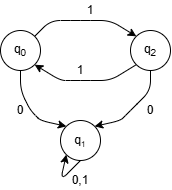
\includegraphics[width=0.3\textwidth]{Images/dfagraph.png}
                \end{center}
                Oppure dando una matrice di transizione
                \begin{center}
                    \begin{tabular}{|c|c|c|}
                        \hline
                         & 0 & 1 \\
                        \hline
                        $\displaystyle \to q_0$ & $q_1$ & $q_2$\\
                        \hline
                        $*q_1$& $q_1$ & $q_1$ \\
                        \hline
                        $q_2$ & $q_1$ & $q_0$ \\
                        \hline
                    \end{tabular}
                \end{center}
                Dove lo stato iniziale è indicato con $\to$ e lo stato finale con $*$.
                \begin{definitionbox}{Automa a stato finito non deterministico (NFA)}{}
                    E' una quintupla $\mathcal{M}=\langle Q,\Sigma, \delta, q_0, F\rangle$ dove $\delta:Q\times\Sigma\to\wp(Q)$.\\
                    $\wp(Q)$ mappa un \textbf{insieme di stati}, cioè l'insieme di tutti i sottoinsiemi possibili di $Q$. Ad esempio se abbiamo $Q=\{q_0,q_1,q_2\}$, $\wp(Q)=\left\{\{q_0\},\{q_1\},\{q_2\},\{q_0,q_1\},\ldots,\{q_0,q_1,q_2\}\right\}$
                \end{definitionbox}
                Analogamente ai DFA, un NFA può essere rappresentato in due modi principali:
                \begin{itemize}
                    \item \textbf{Grafo di transizione}: rimane concettualmente la stessa dei DFA
                    \item \textbf{Tabella di transizione}: ogni casella della tabella (corrispondente a una coppia stato/simbolo) può contenere un insieme di stati \begin{center}
                        \begin{tabular}{|c|c|c|}
                            \hline
                             & 0 & 1\\
                             \hline
                             $\to q_0$ & $\{q_0,q_1\}$ & $q_0$\\
                             \hline
                             $q_1$ & $\emptyset$ & $q_2$\\
                             \hline
                             $*q_2$ & $q_2$ & $q_2$\\
                            \hline
                        \end{tabular}
                    \end{center}
                \end{itemize}
                Il comportamento di un NFA è descritto da un sistema di transizione:
                \begin{itemize}
                    \item \textbf{Configurazioni}: Sono della forma $\langle q, u \rangle$, dove $q \in Q$ è lo stato corrente e $u \in \Sigma^*$ è la stringa ancora da leggere
                    \item \textbf{Relazione di riduzione}: È definita come: $\langle q, \sigma u \rangle \to \langle q', u \rangle$ se $q' \in \delta(q, \sigma)$. \textbf{Non è deterministica} ma comunque \textbf{terminante}, poichè a ogni passo viene consumato un simbolo di input (a meno che non si blocchi)
                    \item \textbf{Configurazioni di arresto}: Un NFA può bloccarsi in due modi: \begin{enumerate}
                        \item Quando ha letto tutta la stringa: $\langle q, \varepsilon \rangle$
                        \item Quando si trova in una configurazione $\langle q, \sigma u \rangle$ ma non esistono transizioni possibili per il simbolo $\sigma$ dallo stato $q$ (cioè $\delta(q, \sigma) = \emptyset$)
                    \end{enumerate}
                    \item \textbf{Direttive di Input/Output}: Le direttive di input/output sono simili a quelle dei DFA: \begin{itemize}
                        \item \textbf{Input}: $f_{IN}(u) = \langle q_0, u \rangle$
                        \item \textbf{Output}: $f_{OUT}=\begin{cases}
                            \langle q, u \rangle = \text{True} & \text{se }q \in F, u = \varepsilon\\
                            \text{False} & \text{altrimenti}
                        \end{cases}$
                    \end{itemize}
                    \item \textbf{Linguaggio Accettato}: Il linguaggio $L(\mathcal{M})$ accettato (o riconosciuto) da un NFA $\mathcal{M}$ è l'insieme delle stringhe $u$ per cui esiste almeno una computazione che, partendo dalla configurazione iniziale $\langle q_0, u \rangle$, raggiunge una configurazione $\langle q, \varepsilon \rangle$ dove $q$ è uno stato finale. Questo è un punto chiave del non determinismo: basta una computazione accettante tra tutte quelle possibili.\\
                    Un modo equivalente per definire il linguaggio accettato usa la funzione estesa $\hat{\delta} : Q \times \Sigma^* \to \wp(Q)$: \begin{itemize}
                        \item $\hat{\delta}(q, \varepsilon) = {q}$
                        \item $\hat{\delta}(q, u\sigma) = \bigcup_{q' \in \hat{\delta}(q, u)} \delta(q', \sigma)$
                    \end{itemize}
                    Con questa definizione, una stringa $u$ è accettata se e solo se esiste uno stato $q$ nell'insieme $\hat{\delta}(q_0, u)$ che sia uno stato finale ($q \in F$). In altre parole, $L(\mathcal{M}) = {u \mid \hat{\delta}(q_0, u) \cap F \neq \emptyset }$
                \end{itemize}
                \begin{theorembox}{Rabin-Scott}{}
                    Sia $\mathcal{M}=\langle Q,\Sigma,\delta_N,q_0,F_N\rangle$ un NFA. Allora esiste un DFA $\mathcal{M}_D$ tale che $L(\mathcal{M}_D)=L(\mathcal{M})$
                \end{theorembox}
                \textbf{Prova}: Costruiamo $\mathcal{M}_D$ come la quintupla $\langle\wp(Q),\Sigma,\delta_D,\{q_0\},F_D\rangle$. L'idea centrale della costruzione è che ogni stato del nuovo DFA $\mathcal{M}_D$ corrisponde a un insieme di stati dell'NFA originale.
                \begin{itemize}
                    \item $Q_D=\wp(Q_N)$: questo significa che ogni stato del DFA è un sottoinsieme degli stati dell'NFA. Se l'NFA ha $|Q_N|$ stati, il DFA risultante può avere fino a $2^{|Q_N|}$ stati, sebbene non tutti siano necessariamente raggiungibili.
                    \item $\delta_D$: per ogni stato $q_D\in\wp(Q_N)$ (che è un insieme di stati dell'NFA) e per ogni simbolo $\sigma \in \Sigma$, la transizione $\delta_D(q_D, \sigma)$ porta a un nuovo stato del DFA che è l'unione di tutti gli stati raggiungibili nell'NFA da qualsiasi stato in $q_D$ leggendo $\sigma$. Formalmente: \begin{equation*}
                        \delta_D(q_D, \sigma) = \bigcup_{q \in q_D} \delta_N(q, \sigma)
                    \end{equation*}
                    \item $F_D$: Uno stato $q_D \subseteq Q_N$ del DFA è uno stato finale se e solo se contiene almeno uno stato finale dell'NFA. Formalmente: \begin{equation*}
                        F_D = {q_D \subseteq Q_N \mid q_D \cap F_N \neq \emptyset}
                    \end{equation*}
                \end{itemize}
                \begin{example}{}
                    \begin{itemize}
                        \item \textbf{NFA Originale $\left(\mathcal{M}_N\right)$}: $\mathcal{M}=\left(\{q_0,q_1,q_2\},\{0,1\},\delta_N,q_0,q_2\right)$ con \begin{center}
                            $\delta_N=$ \begin{tabular}{|c|c|c|}
                                \hline
                                & 0 & 1 \\
                                \hline
                                $\to q_0$ & $q_0$ & $\{q_0,q_1\}$\\
                                \hline
                                $q_1$ & $\emptyset$ & $q_2$\\
                                \hline
                                $*q_2$ & $q_2$ & $q_2$\\
                                \hline
                            \end{tabular}
                        \end{center}
                        \item \textbf{DFA Derivante $(\mathcal{M}_D)$}: $\mathcal{M}_D=(Q_D,\{0,1\},\delta_D,q_0,F_D)$ \begin{itemize}
                            \item $Q_D=\{\emptyset,\{q_0\},\{q_1\},\{q_2\},\{q_0,q_1\},\{q_0,q_2\},\{q_1,q_2\},\{q_0,q_1,q_2\}\}$
                            \item $F_D=\{\{q_2\},\{q_0,q_2\},\{q_1,q_2\},\{q_0,q_1,q_2\}\}$ (tutti gli stati che contengono lo stato finale della NFA)
                            \item $\delta_D$: \begin{enumerate}
                                \item \textbf{Da $\{q_0\}$}: \begin{itemize}
                                    \item $\delta_D(q_0,0)=\delta_N(q_0,0)=q_0$
                                    \item $\delta_D(q_0,1)=\delta_N(q_0,1)=\{q_0,q_1\}$
                                \end{itemize}
                                \item \textbf{Da $\{q_0,q_1\}$}: \begin{itemize}
                                    \item $\delta_D(\{q_0,q_1\},0)=\delta_N(q_0,0)\cup \delta_N(q_1,0)=\{q_0\}\cup\emptyset=q_0$
                                    \item $\delta_D(\{q_0,q_1\},1)=\delta_N(q_0,1)\cup \delta_N(q_1,1)=\{q_0,q_1\}\cup\{q_2\}=\{q_0,q_1,q_2\}$ 
                                \end{itemize}
                                \item \textbf{Da $\{q_0,q_1,q_2\}$}: \begin{itemize}
                                    \item $\delta_D(\{q_0,q_1,q_2\},0)=\delta_N(q_0,0)\cup \delta_N(q_1,0)\cup\delta_N(q_2,0)=\{q_0\}\cup\emptyset\cup\{q_2\}=\{q_0,q_2\}$
                                    \item $\delta_D(\{q_0,q_1,q_2\},1)=\delta_N(q_0,1)\cup \delta_N(q_1,1)\cup\delta_N(q_2,1)=\{q_0,q_1\}\cup\{q_2\}\cup\{q_2\}=\{q_0,q_1,q_2\}$
                                \end{itemize}
                                \item \textbf{Da $\{q_0,q_2\}$}: \begin{itemize}
                                    \item $\delta_D(\{q_0,q_2\},0)=\delta_N(q_0,0)\cup \delta_N(q_2,0)=\{q_0\}\cup\{q_2\}=\{q_0,q_2\}$
                                    \item $\delta_D(\{q_0,q_2\},1)=\delta_N(q_0,1)\cup \delta_N(q_2,1)=\{q_0,q_1\}\cup\{q_2\}=\{q_0,q_1,q_2\}$
                                \end{itemize}
                            \end{enumerate}
                            Quindi \begin{center}
                                $\delta_D=$ \begin{tabular}{|c|c|c|}
                                \hline
                                & 0 & 1 \\
                                \hline
                                $\to q_0$ & $q_0$ & $\{q_0,q_1\}$\\
                                \hline
                                $\{q_0,q_1\}$ & $q_0$ & $\{q_0,q_1,q_2\}$\\
                                \hline
                                $*\{q_0,q_1,q_2\}$ & $\{q_0,q_2\}$ & $\{q_0,q_1,q_2\}$\\
                                \hline
                                $*\{q_0,q_2\}$ & $\{q_0,q_2\}$ & $\{q_0,q_1,q_2\}$\\
                                \hline
                            \end{tabular}
                            \end{center}
                        \end{itemize}
                    \end{itemize}
                    \textit{Abbiamo costruito la tabella includendo unicamente gli stati raggiungibili a partire da $\{q_0\}$. Secondo la definizione di $\delta_D$, non è necessario calcolare le transizioni per stati come $\{q_1\}$, $\{q_1,q_2\}$ e $\{q_2\}$, dato che non vengono mai raggiunti.}
                \end{example}
                \begin{demonstration}
                    \large\textbf{Dimostrazione per induzione}\normalsize\\
                    \textbf{Base}
                    \begin{itemize}
                        \item Per la definizione della funzione di transizione estesa in un DFA, $\hat{\delta}_D({q_0}, \varepsilon) = {q_0}$
                        \item Per la definizione della funzione di transizione estesa in un NFA, $\hat{\delta}_N(q_0, \varepsilon) = {q_0}$
                    \end{itemize}
                    Quindi, la condizione è soddisfatta per la stringa vuota: $\hat{\delta}_D({q_0}, \varepsilon) = \hat{\delta}_N(q_0, \varepsilon)$.\\
                    \textbf{Passo (Stringa $u\sigma$)}
                    \begin{itemize}
                        \item Assumiamo, per ipotesi induttiva, che per una generica stringa $u$, valga $\hat{\delta}_D({q_0}, u) = \hat{\delta}_N(q_0, u)$, vogliamo dimostrare che la stessa uguaglianza vale per la stringa $u\sigma$
                        \item Applichiamo la definizione di $\hat{\delta}_D$ a $u\sigma$: $\hat{\delta}_D({q_0}, u\sigma) = \delta_D(\hat{\delta}_D({q_0}, u), \sigma)$, possiamo sostituire $\hat{\delta}_D({q_0}, u)$ con $\hat{\delta}_N(q_0, u)$: $= \delta_D(\hat{\delta}_N(q_0, u), \sigma)$
                        \item Ora applichiamo la definizione di $\delta_D$: è l'unione delle transizioni $\delta_N(q', \sigma)$ per tutti gli stati $q'$ nell'insieme $\hat{\delta}_N(q_0, u)$:$= \bigcup_{q' \in \hat{\delta}_N(q_0, u)} \delta_N(q', \sigma)$. Questa è precisamente la definizione di $\hat{\delta}_N(q_0, u\sigma)$
                    \end{itemize}
                    Quindi, $\hat{\delta}_D({q_0}, u\sigma) = \hat{\delta}_N(q_0, u\sigma)$.\\
                    Avendo dimostrato per induzione che $\hat{\delta}_D({q_0}, u) = \hat{\delta}_N(q_0, u)$ per ogni stringa $u \in \Sigma^*$, possiamo concludere sull'accettazione del linguaggio:
                    \begin{itemize}
                        \item Una stringa $u$ è accettata dal DFA $\mathcal{M}_D$ se e solo se $\hat{\delta}_D({q_0}, u) \in F_D$
                        \item Per definizione di $F_D$, ciò significa che $\hat{\delta}_D({q_0}, u)$ deve contenere almeno uno stato finale di $\mathcal{M}_N$, ovvero $\hat{\delta}_D({q_0}, u) \cap F_N \neq \emptyset$
                        \item Poiché $\hat{\delta}_D({q_0}, u) = \hat{\delta}_N(q_0, u)$, questo è equivalente a $\hat{\delta}_N(q_0, u) \cap F_N \neq \emptyset$
                        \item E quest'ultima è la condizione di accettazione di una stringa per un NFA $\mathcal{M}_N$
                    \end{itemize}
                    Pertanto, $u$ è accettata da $\mathcal{M}_D$ se e solo se è accettata da $\mathcal{M}_N$, il che significa che $L(\mathcal{M}_D) = L(\mathcal{M}_N)$.
                \end{demonstration}
                \begin{definitionbox}{$\varepsilon$-NFA o NFA con transizioni silenti}{}
                    E' una quintupla $M = \langle Q, \Sigma, \delta, q_0, F \rangle$ dove la funzione di transizione, che ha la forma \begin{equation*}
                        \delta : Q \times (\Sigma \cup \{\varepsilon\}) \to \wp(Q)
                    \end{equation*}
                    La peculiarità di questa definizione è l'inclusione di $\varepsilon$ nell'alfabeto di input della funzione di transizione, il che consente transizioni tra stati senza consumare alcun simbolo di input (transizioni silenti). Questo permette, in molti casi, di costruire automi più semplici e leggibili
                \end{definitionbox}
                Il comportamento di un $\varepsilon$-NFA è descritto da un sistema di transizione con le seguenti caratteristiche:
                \begin{itemize}
                    \item \textbf{Configurazioni}: Sono della forma $\langle q, u \rangle$, dove $q \in Q$ è lo stato corrente e $u \in \Sigma^*$ è la stringa ancora da leggere
                    \item \textbf{Relazione di riduzione}: È definita in due modi: \begin{itemize}
                        \item $\langle q, \sigma u \rangle \to \langle q', u \rangle$ se $q' \in \delta(q, \sigma)$ (transizione standard, consumando un simbolo)
                        \item $\langle q, u \rangle \to \langle q', u \rangle$ se $q' \in \delta(q, \varepsilon)$ (transizione silente, senza consumare simboli)
                    \end{itemize}
                    La relazione di riduzione è non deterministica, anche per via della possibilità di scegliere tra leggere o non leggere un simbolo. È generalmente non terminante, ma le computazioni infinite sono dovute solo a cicli di transizioni $\varepsilon$ dallo stesso stato, che possono essere eliminati.
                    \item \textbf{Configurazione di arresto}: Oltre alle configurazioni della forma $\langle q, \varepsilon \rangle$, includono anche quelle in cui l'automa si blocca perché non ci sono transizioni possibili (né con simboli di input, né silenti) da un dato stato con il simbolo corrente
                    \item \textbf{Linguaggio accettato}: Le direttive di input/output sono le stesse degli NFA. Una stringa $u$ è accettata se esiste almeno una computazione che, partendo dalla configurazione iniziale $\langle q_0, u \rangle$, raggiunge una configurazione $\langle q, \varepsilon \rangle$ dove $q$ è uno stato finale. Un modo equivalente per definire il linguaggio accettato utilizza la funzione di transizione estesa $\hat{\delta} : Q \times \Sigma^* \to \wp(Q)$, che si basa sul concetto di $\varepsilon$-closure: \begin{itemize}
                        \item \textbf{$\varepsilon-closure(q)$}: È l'insieme di tutti gli stati raggiungibili da $q$ utilizzando zero o più transizioni $\varepsilon$. Formalmente, include $q$ stesso, tutti gli stati raggiungibili da $q$ tramite $\delta(q, \varepsilon)$, e ricorsivamente tutti gli stati raggiungibili da questi ultimi tramite ulteriori transizioni $\varepsilon$
                        \item \textbf{Funzione di transizione estesa $\hat{\delta}$}: \begin{itemize}
                            \item $\hat{\delta}(q, \varepsilon) = \varepsilon\text{-closure}(q)$
                            \item $\hat{\delta}(q, u\sigma) = \bigcup_{q' \in \hat{\delta}(q, u)} \varepsilon\text{-closure}(\delta(q', \sigma))$
                        \end{itemize}
                        Una stringa $u$ è accettata se e solo se l'insieme di stati raggiungibili dopo aver letto $u$ (cioè $\hat{\delta}(q_0, u)$) contiene almeno uno stato finale ($\hat{\delta}(q_0, u) \cap F \neq \emptyset$)
                    \end{itemize}
                \end{itemize}
                \begin{example}
                    $\mathcal{M}_N=(\{q_0,q_1,q_2\},\{a,b\},\delta_N,q_0,F_N)$
                    \begin{center}
                        $\delta_N=$ \begin{tabular}{|c|c|c|c|}
                            \hline
                             & a & b & $\varepsilon$\\
                            \hline
                            $\to q_0$ & \ldots & \ldots & $q_1$\\
                            \hline
                            $q_1$ & \ldots & \ldots & $q_2$\\
                            \hline
                            $*q_2$ & \ldots & \ldots & $q_1$\\
                            \hline
                        \end{tabular}
                    \end{center}
                    \textbf{Calcolo le $\varepsilon-closure$}: \begin{itemize}
                        \item $\varepsilon-closure(q_0)=\{q_0,q_1,q_2\}$
                        \item $\varepsilon-closure(q_1)=\{q_1,q_2\}$
                        \item $\varepsilon-closure(q_2)=\{q_2,q_1\}$
                    \end{itemize}
                \end{example}
                \begin{algorithm}
                    Per trovare un NFA senza transizioni $\varepsilon$ equivalente:
                    \begin{enumerate}
                        \item Tabelliamo $\delta$ (le funzioni di transizione) dell'automa originale
                        \item Scriviamo il nuovo automa nella forma $\mathcal{M'}=\langle Q',\Sigma,\delta',q_0,F'\rangle$ dove: \begin{itemize}
                            \item $Q'=Q$ (solitamente)
                            \item $\Sigma$ è l'alfabeto
                            \item $\delta'$ sarà la nuova tabella le cui righe si troveranno facendo $\delta'(q,\sigma)=\bigcup_{s\in\delta(q,\sigma)}\varepsilon-closure(s)$
                            \item $q_0$ stato iniziale (solitamente è lo stesso)
                            \item $F'$ è l'insieme di tutti gli stati che hanno nella propria $\varepsilon$-closure uno stato finale dell'automa originale
                        \end{itemize}
                    \end{enumerate}
                \end{algorithm}
        \section{Minimizzazione di DFA}
            La minimizzazione di un DFA mira a trovare un automa equivalente, che accetti lo stesso linguaggio, ma con il numero minimo di stati.
            \begin{itemize}
                \item \textbf{Stati indistinguibili ($q\sim q'$)}: sono considerati indistinguibili (o equivalenti) se il linguaggio accettato a partire da $q$ è identico al linguaggio accettato a partire da $q'$. Ciò significa che per qualsiasi stringa $u\in\Sigma^*$, se $\hat{\delta}(q,u)\in F$ allora anche $\hat{\delta}(q',u)\text{ (deve) }\in F$ e viceversa. Questa relazione di indistinguibilità è una relazione di equivalenza.
                \item \textbf{Classe di equivalenza ($\equivalenceclass{q}$)}: è l'insieme di tutti gli elementi di $Q$ che sono in relazione con $q$ ($\forall x\in Q, x\sim q$)
                \item \textbf{Quoziente di $Q$ ($\quotientof{Q}$)}: è l'insieme i cui elementi sono le classi di equivalenza stesse,\\
                $\quotientof{Q}=\{\equivalenceclass{q}\mid q\in Q\}$
            \end{itemize}
            \underline{Due stati indistinguibili possono intuitivamente essere trasformati in un unico stato}.\\
            Quindi:
            \begin{equation*}
                \mathcal{M'}=\langle\quotientof{Q},\Sigma,\delta',\equivalenceclass{q_0},F'\rangle
            \end{equation*}
            \subsection{Algoritmo}
                \begin{enumerate}
                    \item Suddividiamo gli stati in due classi di equivalenza: quelli finali e quelli non finali
                    \item A ogni passo consideriamo le classi di equivalenza ottenute al passo precedente \begin{enumerate}
                        \item  Per ognuna di esse immaginiamo che tutti gli stati all'interno leggano un $\sigma$
                        \item Se tutti gli stati finiscono in altri stati della stessa classe di equivalenza, allora questi stati sono ancora considerati simili per quel $\sigma$
                        \item Altrimenti quei due stati non sono più indistinguibili. A questo punto la classe di equivalenza viene suddivisa in sottogruppi più piccoli, separando gli stati che si comportano in modo diverso
                    \end{enumerate}
                    \item Torniamo al punto (2.) e ripetiamo il processo, l'algoritmo si ferma solo quando, dopo aver controllato tutti i grupi con tutti i simboli, non c'è più nulla da dividere 
                \end{enumerate}
                \begin{lstlisting}
                ind = {insieme di (q,q') indistinguibili};
                old_ind = null;
                while(ind != old_ind) {
                    old_ind = ind;
                    ind = null;
                    for each (q,q') in old_ind {
                        ok = true;
                        for simb in alfabeto {
                            if(!indistinguibili(delta(q,simb),delta(q',simb))){
                                ok = false;
                                break;
                            }
                        }
                        if (ok) {
                            ind = ind + (q,q');
                        }
                    }
                }
                \end{lstlisting}
                \begin{example}
                    Consideriamo il seguente DFA:
                    \begin{center}
                        \begin{tabular}{|c|c|c|}
                            \hline
                            & \textbf{a} & \textbf{b}\\
                            \hline
                            $\to q_0$ & $q_0$ & $q_1$ \\
                            \hline
                            $q_1$ & $q_1$ & $q_2$ \\
                            \hline
                            $q_2$ & $q_2$ & $q_3$ \\
                            \hline
                            $*q_3$ & $q_3$ & $q_3$ \\
                            \hline
                        \end{tabular}
                    \end{center}
                    \begin{enumerate}
                        \item $\sim\,=\{\{q_3\},\{q_0,q_1,q_2\}\}$
                        \item \textbf{Prima iterazione}: \begin{enumerate}
                            \item Consideriamo $\{q_0,q_1,q_2\}$
                            \item Leggiamo 'a': \begin{enumerate}
                                \item $\delta(q_0,a)=q_0 \in \{q_0,q_1,q_2\}$
                                \item $\delta(q_1,a)=q_1 \in \{q_0,q_1,q_2\}$
                                \item $\delta(q_2,a)=q_2 \in \{q_0,q_1,q_2\}$
                            \end{enumerate}
                            \item Leggiamo 'b': \begin{enumerate}
                                \item $\delta(q_0,b)=q_1 \in \{q_0,q_1,q_2\}$
                                \item $\delta(q_1,b)=q_2 \in \{q_0,q_1,q_2\}$
                                \item $\delta(q_2,b)=q_3 \notin \{q_0,q_1,q_2\}$
                            \end{enumerate}
                            \item Quindi $\sim\,=\{\{q_3\},\{q_0,q_1\},\{q_2\}\}$
                        \end{enumerate}
                        \item \textbf{Seconda iterazione}: \begin{enumerate}
                            \item Consideriamo $\{q_0,q_1\}$
                            \item Leggiamo 'a': \begin{enumerate}
                                \item $\delta(q_0,a)=q_0 \in \{q_0,q_1\}$
                                \item $\delta(q_1,a)=q_1 \in \{q_0,q_1\}$
                            \end{enumerate}
                            \item Leggiamo 'b': \begin{enumerate}
                                \item $\delta(q_0,b)=q_1 \in \{q_0,q_1\}$
                                \item $\delta(q_1,b)=q_2 \notin \{q_0,q_1\}$
                            \end{enumerate}
                            \item Quindi $\sim\,=\{\{q_3\},\{q_0\},\{q_1\},\{q_2\}\}$
                        \end{enumerate}
                    \end{enumerate}
                    Quindi il DFA era già minimo.
                \end{example}
                \begin{example}
                    \begin{center}
                        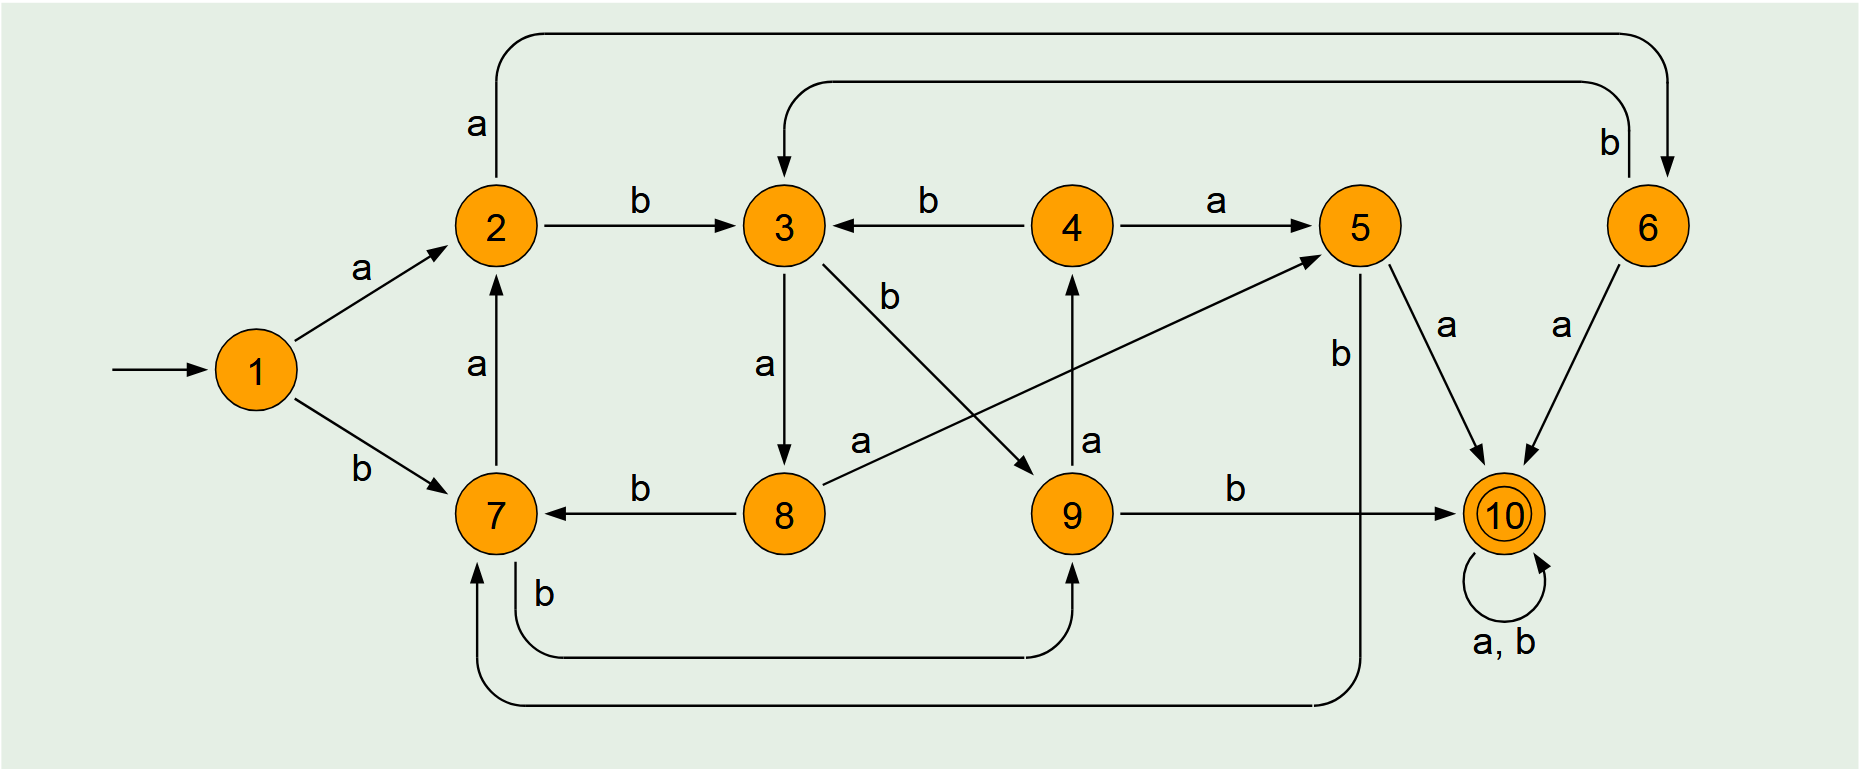
\includegraphics[width=0.8\textwidth]{Images/minimizzazionefebbraio2024.png}
                    \end{center}
                    \footnotesize
                    \begin{enumerate}
                        \item Costruiamo la tabella di transizione (non necessaria ma aiuta): \begin{center}
                            \begin{tabular}{|c|c|c|}
                                \hline
                                & \textbf{a} & \textbf{b}\\
                                \hline
                                $\to$1 & 2 & 7\\
                                \hline
                                2 & 6 & 3 \\
                                \hline
                                7 & 2 & 9\\
                                \hline
                                6 & 10 & 3\\
                                \hline
                                3 & 8 & 9\\
                                \hline
                                9 & 4 & 10\\
                                \hline
                                $*$10 & 10 & 10\\
                                \hline
                                8 & 5 & 7\\
                                \hline
                                4 & 5 & 3\\
                                \hline
                                5 & 10 & 7\\
                                \hline
                            \end{tabular}
                        \end{center}
                        \item $\sim\,=\{\{10\},\{1,2,3,4,5,6,7,8,9\}\}$
                        \item \textbf{Prima iterazione}: \begin{enumerate}
                            \item Consideriamo $\{1,2,3,4,5,6,7,8,9\}$
                            \item Leggiamo 'a': \begin{enumerate}
                                \item $\delta(1,a)=2$
                                \item $\delta(2,a)=6$
                                \item $\delta(3,a)=8$
                                \item $\delta(4,a)=5$
                                \item $\delta(5,a)=10\notin\{1,2,3,4,5,6,7,8,9\}$
                                \item $\delta(6,a)=10\notin\{1,2,3,4,5,6,7,8,9\}$
                                \item $\delta(7,a)=2$
                                \item $\delta(8,a)=5$
                                \item $\delta(9,a)=4$
                            \end{enumerate}
                            \item Leggiamo 'b': \begin{enumerate}
                                \item $\delta(1,b)=7$
                                \item $\delta(2,b)=3$
                                \item $\delta(3,b)=9$
                                \item $\delta(4,b)=3$
                                \item $\delta(7,b)=9$
                                \item $\delta(8,b)=7$
                                \item $\delta(9,b)=10\notin\{1,2,3,4,5,6,7,8,9\}$
                            \end{enumerate}
                            \item Quindi $\sim\,=\{\{10\},\{5,6\},\{9\},\{1,2,3,4,7,8\}\}$
                        \end{enumerate}
                        \item Nella seconda (e ultima in questo caso) iterazione avremo che $\sim\,=\{\{10\},\{5,6\},\{9\},\{1\},\{2,4,8\},\{3,7\}\}$
                    \end{enumerate}
                \end{example}
            \subsection{Espressioni regolari}
                \begin{definitionbox}{}{}
                    Un'espressione regolare è una stringa che descrive schematicamente un insieme di stringhe. I linguaggi denotati dalle RE sono definiti induttivamente: 
                    \begin{itemize}
                        \item $\emptyset$ è una RE che denota il linguaggio vuoto
                        \item $\varepsilon$ è una RE che denota il linguaggio contenente solo la stringa vuota $\{\varepsilon\}$
                        \item Per ogni simbolo $\sigma\in\Sigma$, $\sigma$ è una RE che denota il linguaggio $\{\sigma\}$
                        \item Se $r_1$ è un'espressione regolare che denota il linguaggio $L_1$ e $r_2$ denota $L_2$, allora: \begin{itemize}
                            \item $r_1+r_2$ (o $r_1\mid r_2$) denota l'unione dei linguaggi $L_1\cup L_2$
                            \item $r_1r_2$ denota la concatenazione dei linguaggi $L_1\cdot L_2$
                        \end{itemize}
                        \item Se $r$ è un'espressione regolare che denota $L$, $r^*$ denota la chiusura di Kleene $L^*$
                    \end{itemize}
                \end{definitionbox}
        \section{Proprietà dei linguaggi regolari}
            \begin{itemize}
                \item \textbf{Unione}: Se $L$ e $L'$ sono linguaggi regolari, anche la loro unione ($L \cup L'$) è un linguaggio regolare. Questa proprietà è "ovvia per definizione" in relazione alle espressioni regolari.
                \item \textbf{Concatenazione}: Se $L$ e $L'$ sono linguaggi regolari, anche la loro concatenazione ($L \cdot L'$) è un linguaggio regolare. Anche questa è "ovvia per definizione".
                \item \textbf{Chiusura di Kleene}: Se $L$ è un linguaggio regolare, anche la sua chiusura di Kleene ($L^*$) è un linguaggio regolare. Questa proprietà è anch'essa "ovvia per definizione".
                \item \textbf{Complementazione}: Se $L$ è un linguaggio regolare su un alfabeto $\Sigma$, allora anche il suo complementare ($\overline{L} = \Sigma^* \setminus L$) è regolare. Questo si dimostra prendendo un DFA che riconosce $L$ e scambiando gli stati finali con quelli non finali.
                \item \textbf{Intersezione}: Se $L$ e $L'$ sono linguaggi regolari, allora anche la loro intersezione ($L \cap L'$) è un linguaggio regolare. La chiusura rispetto all'intersezione si deduce facilmente dalla chiusura per complementazione, dato che $L \cap L' = \overline{\overline{L} \cup \overline{L'}}$.
            \end{itemize}
            \subsection{Pumping Lemma}
                \begin{theorembox}{Pumping Lemma}{}
                    Sia $L$ un linguaggio regolare. Allora esiste una costante $n\in\mathbb{N}$ (detta "lunghezza di pompaggio" o "numero di stati del DFA") tale che, per ogni $z\in L$ con $|z|\geq n$, possiamo decomporre $z$ come $uvw$ in modo che: \begin{itemize}
                        \item $|uv|\geq n$ (la porzione "pompabile" $v$ deve trovarsi entro i primi $n$ simboli della stringa)
                        \item $|v|>0$ (la porzione "pompabile" non deve essere vuota)
                        \item per ogni $i\geq 0$ si ha che $uv^iw\in L$ ($v$ può essere ripetuta $i$ volte, inclusa l'eliminazione $i=0$, e la stringa rimarrà nel linguaggio)
                    \end{itemize}
                \end{theorembox}
                \begin{demonstration}
                    \begin{itemize}
                        \item Assumiamo $L$ regolare $\Rightarrow$ per il Pumping Lemma, esiste una costante $n$.
                        \item Si sceglie una stringa $z=\sigma_1\sigma_2\ldots\sigma_{|z|}\in L$ la cui lunghezza $|z|\geq n$.
                        \item Dato che la stringa è accettata dall'automaa, abbiamo $q_0\xrightarrow{\sigma_1}q_1\xrightarrow{\sigma_2}\ldots\xrightarrow{\sigma_{|z|}}q_{|z|}=q_F\in F$
                        \item Dato che il DFA ha solo $n$ stati in totale, necessariamente si ha che almeno uno stato $\bar{q}$ viene attraversato due volte nei primi $n$ passi, ossia $\bar{q}=q_i=q_j$ per qualche $0\leq i<j\leq n$
                        \item \textbf{Decomposizione di z}: \begin{itemize}
                            \item $u=\sigma_1\ldots\sigma_i$
                            \item $v=\sigma_{i+1}\ldots\sigma_j$
                            \item $w=\sigma_{j+1}\ldots\sigma_{|z|}$
                        \end{itemize}
                        si ha $q_0\xrightarrow{u}\bar{q}\xrightarrow{v}\bar{q}\xrightarrow{w}q_F$, quindi $q_0\xrightarrow{u}\bar{q}\xrightarrow{v^i}\bar{q}\xrightarrow{w}q_F$ perchè $\bar{q}\xrightarrow{v}\bar{q}$
                    \end{itemize}
                \end{demonstration}

                Il pumping lemma viene tipicamente utilizzato per provare che un linguaggio $L$ \textbf{non} è regolare.\\
                A tale scopo: \begin{itemize}
                    \item Si sceglie un numero arbitrario $n$
                    \item Si trova una stringa $z\in L$, con lunghezza $|z|\geq n$
                    \item Si dimostra che, per ogni modo in cui si può dividere $z$ in tre parti $uvw$ (dove $|uv|\leq n$ e $|v|>0$), se si ripete la parte $v$ (o la si elimina), la stringa che si ottiene \textbf{non} appartiene più al linguaggio
                \end{itemize}
                Questo contraddice la definizione di linguaggio regolare, provando così che il linguaggio non lo è.
                \begin{example}
                    Possiamo dimostrare, utilizzando il pumping lemma, che il linguaggio $\{0^n1^n\}$ non è regolare. Infatti, preso $n$ arbitrario, consideriamo la stringa $0^n1^n$. Decomponendo tale stringa in tre parti $u, v, w$ tali che la lunghezza delle prime due sia $\leq n$ e la seconda sia non vuota, si ha chiaramente $u = 0^a$, $v = 0^b$ e $w = 0^c1^n$ con $a+b+c = n$, $b > 0$. Allora, per esempio per $i = 0$, si ha che $uv^0w = 0^a0^c1^n$ non appartiene al linguaggio in quanto $a+c < n$.
                \end{example}
        \section{Automi a pila}
            \begin{definitionbox}{Automa a pila non deterministico (PDA)}{}
                E' una tupla \begin{equation*}
                    \mathcal{M}=\langle Q,\Sigma,\Gamma,\delta,q_0,Z,F\rangle
                \end{equation*}
                \begin{itemize}
                    \item $Q,\Sigma,q_0,F$ come per gli automi a stati finiti
                    \item $\Gamma$: alfabeto della pila
                    \item $Z$: simbolo inziale della pila
                    \item $\delta:Q\times(\Sigma\cup\{\varepsilon\})\times\Gamma\to\wp_F(Q\times\Gamma^*)$, dove $\wp_F(X)$ denota l'insieme dei sottoinsiemi \textit{finiti} di $X$
                \end{itemize}
            \end{definitionbox}
            In termini informali, quando un automa a pila si trova nello stato $q$, legge un simbolo $\sigma$ (o esegue una transizione silente) e rimuove il simbolo in cima $Z$ dalla pila, può passare a un nuovo stato $q'$ e inserire una sequenza $\alpha$ (anche vuota) di nuovi simboli in cima alla pila.\\
            L'automa è \textbf{non deterministico}, il che significa che per la stessa combinazione di stato, simbolo di input corrente e simbolo in cima alla pila, possono esserci diverse transizioni possibili.
            Il comportamento di un PDA è descritto da un sistema di transizione con le seguenti caratteristiche:
            \begin{itemize}
                \item \textbf{Configurazioni}: sono nella forma $\langle q,u,\alpha\rangle$ dove $q\in Q$ è lo stato corrente, $u\in\Sigma^*$ è la stringa ancora da leggere e $\alpha\in\Gamma^*$ è il contenuto corrente della pila
                \item \textbf{Relazione di riduzione}: Descrive come la macchina si muove da una configurazione all'altra: \begin{itemize}
                    \item $\langle q, \sigma u, X \alpha \rangle \rightarrow \langle q', u, \gamma \alpha \rangle$ se $\langle q', \gamma \rangle \in \delta \langle q, \sigma, X \rangle$ (lettura di un simbolo di input $\sigma$)
                    \item $\langle q, u, X \alpha \rangle \rightarrow \langle q', u, \gamma \alpha \rangle$ se $\langle q', \gamma \rangle \in \delta \langle q, \varepsilon, X \rangle$ (transizione silente $\varepsilon$)
                \end{itemize}
                La relazione di riduzione è non deterministica. Ciò significa che per una data configurazione, potrebbero esserci più transizioni possibili, incluse le transizioni silenti. Le computazioni possono essere non terminanti se ci sono cicli di transizioni $\varepsilon$ che non modificano l'input o la pila in modo significativo per il consumo della stringa
                \item \textbf{Configurazioni di arresto}: Si verificano quando non ci sono ulteriori mosse possibili
                \item \textbf{Direttive di Input/Output}: \begin{itemize}
                    \item \textbf{Input}: $f_{IN}(u)=\langle q_0, u, Z \rangle$
                    \item \textbf{Output}: \begin{itemize}
                        \item Riconoscimento per pila vuota (Empty Stack Acceptance): \begin{equation*}
                            f_{OUT}(\langle q, u, \alpha \rangle)= \begin{cases} \text{True} & \text{se } u = \varepsilon \text{ e } \alpha = \varepsilon \\ \text{False} & \text{altrimenti} \end{cases}
                        \end{equation*}
                        \item Riconoscimento per stati finali (Final State Acceptance): \begin{equation*}
                            f_{OUT}(\langle q, u, \alpha \rangle) = \begin{cases} \text{True} & \text{se } u = \varepsilon \text{ e } q \in F \\ \text{False} & \text{altrimenti} \end{cases}
                        \end{equation*}
                    \end{itemize}
                \end{itemize}
                \item \textbf{Linguaggio accettato}: \begin{itemize}
                    \item Per pila vuota: $L(\mathcal{M})=\{u\in\Sigma^*\mid\langle q_0,u,Z\rangle\to^*\langle\_,\varepsilon,\varepsilon\rangle\}$
                    \item Per stati finali: $L(\mathcal{M})=\{u\in\Sigma^*\mid\langle q_0,u,Z\rangle\to^*\langle q,\varepsilon,\_\rangle,q\in F\}$
                \end{itemize}
                Usiamo la wildcar \_ per sottolineare il fatto che lo stato non è rilevante.\\
                \textit{Le due definizioni sono equivalenti: se il linguaggio $L$ è riconosciuto da un qualche PDA secondo la prima definizione, allora esiste anche un PDA che lo riconosce secondo l'altra e viceversa}.
            \end{itemize}
            \begin{definitionbox}{Automa a pila deterministico (DPDA)}{}
                 E' una tupla $\mathcal{M} = \langle Q, \Sigma, \Gamma, \delta, q_0, Z, F \rangle$ dove: \begin{itemize}
                    \item $Q$, $\Sigma$, $q_0$ e $F$ sono come per gli automi a stati finiti
                    \item $\Gamma$ è l'alfabeto della pila
                    \item $Z$ è il simbolo iniziale nella pila
                    \item $\delta : Q \times (\Sigma \cup {\varepsilon}) \times \Gamma \to \mathcal{P}_F(Q \times \Gamma^*)$ soddisfa la seguente condizione di determinismo:
                    \\Per ogni $\langle q, \sigma, X \rangle \in Q \times \Sigma \times \Gamma$: $$|\delta\langle q, \sigma, X \rangle| + |\delta\langle q, \varepsilon, X \rangle| \le 1$$
                 \end{itemize}
                 Questa condizione garantisce che per ogni stato corrente $q$, simbolo di input corrente $\sigma$ (o transizione silente $\varepsilon$), e simbolo in cima alla pila $X$, esista al più una transizione possibile. Non è possibile, ad esempio, leggere un simbolo di input e contemporaneamente avere una transizione silente dallo stesso stato con lo stesso simbolo in cima alla pila.
            \end{definitionbox}
        \section{Linguaggi Context-Free}
        \subsection{Grammatiche Context-Free}
            \begin{definitionbox}{Grammatica CF}{}
                Una CFG è definita da una quadrupla $\langle T, N, P, S \rangle$:
                \begin{itemize}
                    \item $T$ è l'alfabeto dei terminali (i simboli che compongono le stringhe del linguaggio)
                    \item $N$ è l'alfabeto dei non terminali (simboli intermedi usati nelle derivazioni), con $T \cap N = \emptyset$
                    \item $P$ è un insieme finito di produzioni (o regole), della forma $A ::= \alpha$, dove $A \in N$ e $\alpha \in (T \cup N)^*$
                    \item $S \in N$ è il simbolo iniziale (o assioma), da cui partono le derivazioni
                \end{itemize}
            \end{definitionbox}
            \begin{example}
                \begin{itemize}
                    \item $T=\{0,1,\ldots,9\}$
                    \item $N=\{Exp,Num\}$
                    \item $P=\{Exp:=Num, Exp:=(Exp+Exp), Num:=T\}$
                    \item $S=Exp$
                \end{itemize}
            \end{example}
            \begin{definitionbox}{Derivazione in un passo}{}
                Questa nozione è fondamentale per comprendere come una grammatica context-free (CFG) genera le stringhe di un linguaggio.\\
                Si considerano una grammatica $G = \langle T, N, P, S \rangle$. Si prendono due stringhe, $\alpha$ e $\beta$, che possono contenere sia simboli terminali che non terminali (ovvero $\alpha, \beta \in (T \cup N)^*$).\\
                Si dice che $\beta$ è derivabile da $\alpha$ in un passo se valgono le seguenti condizioni: \begin{itemize}
                    \item La stringa $\alpha$ ha la forma $\alpha_1 A \alpha_2$. Questo significa che $\alpha$ contiene un non terminale $A$, circondato da due (eventualmente vuote) sottostringhe $\alpha_1$ e $\alpha_2$, che possono essere composte da terminali e non terminali ($\alpha_1, \alpha_2 \in (T \cup N)^*$)
                    \item La stringa $\beta$ ha la forma $\alpha_1 \gamma \alpha_2$
                    \item Esiste una produzione (regola) $A ::= \gamma$ nell'insieme $P$ delle produzioni della grammatica. Qui $A$ è il non terminale che viene espanso e $\gamma$ è la stringa (di terminali e/o non terminali) con cui $A$ viene sostituito
                \end{itemize}
                 La derivazione in un passo è indicata con $\alpha \to \beta$. Questa relazione è una relazione su $(T \cup N)^*$.
            \end{definitionbox}
            \textbf{Chiusura Riflessiva e transitiva ($\rightarrow^*$)}: \begin{itemize}
                \item La chiusura riflessiva e transitiva di $\rightarrow$ è indicata con $\rightarrow^*$
                \item Si dice che $\beta$ è derivabile da $\alpha$ (in uno o più passi, o anche zero passi se $\alpha = \beta$) se $\alpha \rightarrow^* \beta$
                \item Questa significa che si può ottenere $\beta$ partendo da $\alpha$ attraverso una sequenza di zero o più applicazioni delle regole di derivazione in un passo
            \end{itemize}
            \begin{definitionbox}{Linguaggio generato da una grammatica}{}
                Data una grammatica Context-Free (CF) $G = \langle T, N, P, S \rangle$, il linguaggio generato da $G$, denotato $L(G)$, è definito come l'insieme di tutte le stringhe $u$ che appartengono all'alfabeto dei terminali $T^*$ e che possono essere derivate dal simbolo iniziale $S$: \begin{equation*}
                    L(G)=\{u\in T^*\mid S\to^* u\}
                \end{equation*}
            \end{definitionbox}
            Un linguaggio $L$ è definito Context-Free (CF) se esiste una grammatica CF $G$ che lo genera, ovvero tale che $L(G) = L$.\\
            Talvolta, l'interesse può estendersi non solo al linguaggio generato dall'assioma ($S$), ma a una famiglia di linguaggi generati a partire da ciascun non terminale della grammatica (ad esempio, $L_A(G) = {u \in T^* \mid A \rightarrow^* u}$). In tal caso, la scelta di un assioma specifico non è l'unico aspetto significativo.
        \subsection{Proprietà}
            \begin{definitionbox}{Pumping Lemma}{}
                Se $L$ è un linguaggio CF, esiste una costante $n\in\mathbb{N}$ (lunghezza di pompaggio) tale che, per ogni $z\in L$ con $|z|\geq n$ può essere decomposta in $uvwxy$ in modo che:
                \begin{itemize}
                    \item $|vwx|\geq n$
                    \item $|vx|>0$
                    \item $\forall i\geq 0$ si ha che la stringa $uv^iwx^iy\in L$
                \end{itemize} 
            \end{definitionbox}
            L'idea fondamentale di questo lemma è che, se un linguaggio è CF, allora ogni sua stringa che sia "sufficientemente lunga" può essere divisa in cinque parti. Due di queste parti possono essere ripetute (o eliminate) un numero qualsiasi di volte, e la stringa risultante apparterrà ancora al linguaggio.
            \begin{demonstration}
                \textbf{Prova}: Qualsiasi linguaggio CF (che non includa la stringa vuota $\varepsilon$, per semplicità) può essere generato da una grammatica CF che sia in Forma Normale di Chomsky (CNF). Una grammatica in CNF ha solo due tipi di produzioni (regole di riscrittura): \begin{itemize}
                    \item Un non-terminale che produce due altri non-terminali (es. $A ::= BC$)
                    \item Un non-terminale che produce un singolo simbolo terminale (es. $A ::= \sigma$)
                \end{itemize}
                Proviamo che, per una grammatica in CNF, se un albero di derivazione ha altezza m, allora la stringa finale che genera (la "frontiera" dell'albero) ha una lunghezza massima di $2^{(m-1)}$.\\
                \textbf{Base}: Un albero di altezza 1 significa che il simbolo di partenza ha prodotto direttamente un terminale (es. $S ::= \sigma$). La stringa ha lunghezza 1. E $2^{(1-1)} = 2^0 = 1$. Quindi, il caso base funziona.\\
                \textbf{Passo}: Un albero di altezza $m+1$ significa che il simbolo di partenza ha prodotto due altri non-terminali di altezza $m$ (es. $A::=BC$) le cui stringhe saranno di lunghezza al più $2^{(m-1)}$. Quindi: 
                $$|A|=2^{(m-1)} + 2^{(m-1)}=2^m$$
                Prendiamo $m$ come il numero di non-terminali della grammatica CNF che genera il linguaggio $L$ e stabiliamo $n=2^m$. Data una stringa $z\in L\mid|z|\geq n$, l'altezza del suo albero di derivazione deve essere \textbf{almeno} $m+1$. Visto che l'altezza dell'albero è maggiore del numero di non-terminali, sappiamo sicuramente che un non-terminale compaia due volte in un cammino dalla radice alle foglie (\textbf{Principio dei Cassetti}).
                \begin{itemize}
                    \item Indichiamo con $A^{(1)}$ e $A^{(2)}$ la prima e seconda occorrenza del non-terminale ripetuto
                    \item Supponiamo di avere $z=uvwxy$ dove: \begin{itemize}
                        \item $A^{(1)}$ genera la sottostringa $vwx$
                        \item $A^{(2)}$, contenuta in $A^{(1)}$, genera solo $w$
                        \item Le condizioni del lemma specificano: \begin{itemize}
                            \item $|vwx| \leq n$ perché abbiamo scelto la ripetizione più vicina alle foglie (cioè quella con altezza minore).
                            \item $|vx| > 0$ perché in una grammatica CNF non è possibile che entrambi $v$ e $x$ siano vuoti.
                        \end{itemize}
                    \end{itemize}
                \end{itemize}
                  Poiché $A$ può generare sia $vwx$ che $w$, è possibile ripetere o eliminare $v$ e $x$. Questo significa che le stringhe $uv^iwx^iy$ (per $i \geq 0$) apparterranno tutte al linguaggio.
            \end{demonstration}
            Come nel caso dei regolari, il pumping lemma viene utilizzato per provare che un linguaggio $L$ non è CF.\\
            Per farlo, bisogna scegliere un numero $n$ qualunque, e poi trovare una stringa $z$ che: \begin{itemize}
                \item Appartiene al linguaggio $L$
                \item Ha lunghezza almeno $n$, cioè $|z|\geq n$
            \end{itemize}
            A questo punto, mostriamo che qualunque modo si scelga di dividere $z$ nella forma $$z=uvwxy$$
            rispettando le due condizioni: 
            \begin{itemize}
                \item $|vwx|\leq n$
                \item $|vx|>0$
            \end{itemize}
            allora esiste almeno un valore di $i$ per cui la stringa "pompata"
            $$uv^iwx^iy$$
            non appartiene al linguaggio $L$.
            \begin{example}
                \textit{Provare che $L=\{a^nb^nc^n\}$ non è CF.}
                \begin{enumerate}
                    \item Per assurdo consideriamo $L$ CF
                    \item Scegliamo la stringa "più lunga": $z=a^nb^nc^n$, la lunghezza sarà $|z|=3n\geq n$
                    \item Sappiamo che $z$ può essere decomposta come $uvwxy$
                    \item Applichiamo il lemma: \begin{enumerate}
                        \item $|vwx|\leq n$
                        \item $|vx|>0$
                        \item $\forall i\geq 0, uv^iwx^iy$
                        \item Per certo possiamo dire che $vwx$ non può includere $a$ e $c$ perchè dovrebbe includere tutto $b^n$ e quindi la lunghezza sarebbe in ogni caso $> n$
                        \item Impostiamo $i=0$ (solitamente si usa $i=0$ o $i=2$): $uv^0wx^0y=uwy$ con $|uwy|=|u|+|w|+|y|$
                        \item $|z|=|u|+|v|+|w|+|x|+|y|\Rightarrow |uwy|=|z|-(|v|+|x|)$
                        \item Poichè $|vx|>0$, ne consegue che $|uwy| < |z|$
                    \end{enumerate}
                    \item $L$ non è CF
                \end{enumerate}
            \end{example}
            \subsubsection{Proprietà di Chiusura}
                I linguaggi CF risultano chiusi rispetto a:
                \begin{itemize}
                    \item \textbf{Unione}
                    \item \textbf{Concatenazione}
                    \item \textbf{Chiusura di Kleene}
                \end{itemize}
                I linguaggi CF non risultano chiusi rispetto a:
                \begin{itemize}
                    \item \textbf{Intersezione}
                    \item \textbf{Complementazione}
                \end{itemize}
    \chapter{Teoria della calcolabilità}
        \section{Macchine di Turing}
            \begin{definitionbox}{Macchina di Turing deterministica}{}
                E' una tupla $\mathcal{M}=\langle Q,\Sigma,\Gamma,\delta,q_0,B,F\rangle$ dove:
                \begin{itemize}
                    \item $Q$ è un insieme finito di stati
                    \item $\Sigma$ è un alfabeto di input
                    \item $\Gamma$ è un alfabeto del nastro che include l'alfabeto di input ($\Sigma\subseteq\Gamma$)
                    \item $\delta$ è una funzione di transizione parziale della forma $Q \times \Gamma \to Q \times \Gamma \times \{L,R\}$. Questa funzione specifica l'azione successiva della macchina in base allo stato corrente e al simbolo letto sulla cella del nastro sotto la testina. L'azione consiste nel cambiare stato, scrivere un simbolo su quella cella (scrivere $B$ equivale a cancellare) e spostare la testina a sinistra ($L$) o a destra ($R$). Se per una data combinazione di stato e simbolo non è specificata alcuna azione, la macchina si ferma.
                    \item $q_0$ è lo stato iniziale
                    \item $B$ è un simbolo speciale che appartiene a $\Gamma$ ma non a $\Sigma$ ($B\in\Gamma\smallsetminus\Sigma$). Rappresenta una cella vuota o "blank" sul nastro.
                    \item $F\subseteq Q$ è l'insieme degli stati finali
                \end{itemize}
            \end{definitionbox}
            La scelta di avere due alfabeti e un insieme di stati finali è legata ala visione di una macchina di Turing come \textbf{riconoscitore}.\\
            Una macchina di Turing può essere immaginata come:
            \begin{itemize}
                \item Un nastro, illimitato nei due sensi e suddiviso in celle. Sul nastro è presente un numero finito di simboli diversi da $B$
                \item Una testina (di lettura e scrittura) posizionata su una cella del nastro
                \item La testina si trova in un certo stato $q\in Q$
            \end{itemize}
            \begin{center}
                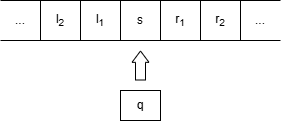
\includegraphics[width=0.5\textwidth]{Images/turingmachine.png}
            \end{center}
            Il funzionamento è determinato dalla funzione di transizione: in ogni istante, in dipendenza deterministica dello stato della testina e del simbolo letto nella cella corrente, la macchina effettua un'azione che comporta: un cambiamento di stato, la scrittura di un simbolo di $\Gamma$ nella cella corrente e lo spostamento della testina a sinistra ($L$) o a destra ($R$) o rimane ferma ($N$).
            \begin{itemize}
                \item \textbf{Configurazioni}: sono rappresentate come $\langle \alpha, q, \beta \rangle$ dove: \begin{itemize}
                    \item $\alpha$ sono i simboli a sinistra della testina
                    \item $q$ è lo stato corrente della testina
                    \item $\beta$ sono i simboli a destra della testina
                \end{itemize}
                Se $\beta$ è vuota, la testina punta a una cella $B$. Viene rappresentata solo la porzione significativa del nastro.
                \item \textbf{Relazione di riduzione}: descrive come le configurazioni cambiano passo dopo passo. Per esempio, se $\delta(q, X) = \langle q', Y, R \rangle$, allora $\langle \alpha, q, X\beta \rangle \to \langle \alpha Y, q', \beta \rangle$ (spostamento a destra). Questa relazione è deterministica e, in generale, non terminante (possono esserci computazioni infinite)
                \item \textbf{Configurazioni di arresto}: sono quelle per cui la funzione di transizione è indefinita (cioè $\delta(q, X)\uparrow$ o $\delta(q, B)\uparrow$)
                \item \textbf{Direttive di Input/Output} \begin{itemize}
                    \item \textbf{Input}: $f_{IN}(u) = \langle \epsilon, q_0, u \rangle$
                    \item \textbf{Output}: $$f_{OUT}(\langle \alpha, q, \beta \rangle)=\begin{cases}
                        \text{True} & \text{se } q\in F\\
                        \text{False} & \text{altrimenti}
                    \end{cases}$$
                \end{itemize}
                \item \textbf{Linguaggio accettato}: è l'insieme di tutte le stringhe $u$ che, partendo dalla configurazione iniziale, possono portare a una configurazione di accettazione. $$L(\mathcal{M}) = \{u \in \Sigma^* \mid \langle \varepsilon, q_0, u \rangle \to^* \langle \alpha, q, \beta \rangle, q \in F\}$$ Il contenuto finale del nastro è irrilevante ai fini dell'accettazione
            \end{itemize}
            \begin{definitionbox}{Linguaggi ricorsivamente enumerabili}{}
                Un linguaggi è \textbf{ricorsivamente enumerabile} se è accettato da una macchina di Turing
            \end{definitionbox}
            \begin{definitionbox}{Linguaggi ricorsivi}{}
                Un linguaggio è \textbf{ricorsivo} se è accettato da una macchina di Turing che termina su ogni input
            \end{definitionbox}
            \subsection{Sintassi del simulatore}
            \begin{verbatim}
                <current state> <read> <write> <dir> <next state>
            \end{verbatim}
            \vspace{-1cm}
            Dove: \begin{itemize}
                \item \texttt{<current state>}: è lo stato corrente (dove si trova la testina)
                \item \texttt{<read>}: è il simbolo che viene letto
                \item \texttt{<write>}: è il simbolo che viene scritto
                \item \texttt{<dir>}: è la direzione $L$ (Sinistra), $R$ (Destra), $*$ (Nessuna)
                \item \texttt{<next state>}: è in quale stato deve andare
            \end{itemize}
            \begin{example}
                \textit{Definire la TM che riconosce il linguaggio regolare $L=\{0^n1^m\mid n,m\geq 0\}$}
                \begin{itemize}
                    \item Leggiamo tutti i simboli 0 spostandoci a destra
                    \item Quando troviamo un 1 cambiamo stato e leggiamo tutti i simboli 1 spostandoci a destra
                    \item Se troviamo $B$ la stringa è accettata, se troviamo 0 la macchina si blocca in uno stato di non accettazione
                \end{itemize}
                Usando la sintassi del simulatore:
                \begin{verbatim}
                    0 0 0 r 0
                    0 1 1 r 1
                    0 _ _ * halt-accept
                    1 1 1 r 1
                    1 _ _ * halt-accept
                \end{verbatim}
                "\_" è Blank
            \end{example}
            \begin{exercise}
                Qui metto un esercizio da esame per costruire una macchina di turing dato un linguaggio
            \end{exercise}        
        \section{Funzioni T-calcolabili}
            Le funzioni T-calcolabili sono quelle funzioni che possono essere calcolate da una Macchina di Turing (TM).\\
            Consideriamo una definizione di TM semplificata: 
            $$\mathcal{M}=\langle Q,\Sigma,\delta,q_0,B\rangle$$
            dove $\Sigma=\Gamma$ include almeno un altro simbolo oltre al blank $B$, e la funzione di transizione $\delta : Q \times \Sigma \to Q \times \Sigma \times \{L,R\}$ è una funzione parziale.\\
            Per calcolare una funzione $f : Input \to Output$, è necessario stabilire un modo per codificare gli elementi del dominio e del codominio come stringhe sul nastro della TM. Questo si realizza tramite due funzioni iniettive: $c_{IN} : Input \to \Sigma^*$ per l'input e $c_{OUT} : Output \to \Sigma^*$ per l'output.
            \begin{itemize}
                \item \textbf{Direttive di Input/Output} \begin{itemize}
                    \item \textbf{Input}: La testina è inizialmente posizionata sul primo simbolo della stringa che rappresenta l'input. La configurazione iniziale per un input $i$ è $f_{IN}(i) = \langle \varepsilon, q_0, c_{IN}(i) \rangle$
                    \item \textbf{Output}: Il risultato della funzione è rappresentato dalla stringa che rimane sul nastro quando l'esecuzione della macchina termina. Se la stringa sul nastro rappresenta effettivamente un risultato valido (secondo la codifica $c_{OUT}$), allora la funzione è definita per quell'input; altrimenti, la funzione risulta indefinita (o "malformata" se si ferma in una configurazione non valida). Formalmente $$f_{OUT}(\langle\alpha,q,\beta\rangle)=\begin{cases}
                        o & \text{se } c_{OUT}(\alpha\beta)=o\\
                        \text{Indefinito} & \text{altrimenti}
                    \end{cases}$$
                \end{itemize}
            \end{itemize}
            \begin{example}
                \textit{Definire una TM che calcola la sommaa di due numeri codificati in unario separati da \#, quindi $1^n\#1^m$ deve dare come output $1^{n+m}$}. L'algoritmo sposta semplicemente tutti gli 1 prima di \# alla fine del secondo argomento cancellando alla fine il separatore.
                \begin{verbatim}
                    0    1 _ r go_r
                    0    # _ r halt
                    go_r 1 1 r go_r
                    go_r # # r go_r
                    go_r _ 1 l go_l
                    go_l 1 1 l go_l
                    go_l # # l go_l
                    go_l _ _ r 0
                \end{verbatim}
            \end{example}
        \section{Tesi di Church-Turing}
            Sebbene le MT non abbiano istruzioni come \texttt{goto} o la possibilità di accedere alla memoria tramite indici come in un linguaggio di programmazione convenzionale, dimostrano una sorprendente potenza espressiva. Concetti come i "salti" possono essere realizzati tramite sequenze di spostamenti elementari della testina sul nastro. Le MT possono essere considerate una versione embrionale dell'architettura di Von Neumann.
            \subsection{La tesi}
                La Tesi di Church-Turing afferma che una funzione è calcolabile con un algoritmo se e solo se è ricorsiva (parziale). Ciò significa che la classe delle funzioni T-calcolabili (quelle calcolabili da una Macchina di Turing) è identificata con la classe intuitiva delle funzioni "calcolabili con un algoritmo". Non può essere dimostrata formalmente. È una congettura che collega una nozione informale e intuitiva ("calcolabile con un algoritmo") a una nozione matematica precisa (funzione ricorsiva o T-calcolabile) però ci sono diversi argomenti significativi che ne rafforzano la validità:
                \begin{itemize}
                    \item \textbf{Equivalenza dei Formalismi}: Tutti i formalismi di calcolo proposti indipendentemente (come le funzioni $\mu$-ricorsive, il lambda-calcolo, le Random Access Machine, le macchine a contatori) si sono dimostrati equivalenti alle Macchine di Turing. Tutti definiscono la stessa classe di funzioni calcolabili, chiamata la classe delle funzioni ricorsive (parziali)
                    \item \textbf{Potere Espressivo}: Ogni funzione che può essere ragionevolmente considerata "algoritmica" si è rivelata appartenere a questa classe
                    \item \textbf{Algoritmi di Trasformazione}: Le dimostrazioni di equivalenza tra formalismi spesso mostrano che esiste un algoritmo che, dato un programma in un formalismo, produce un programma equivalente nel secondo formalismo. Questo implica che ogni formalismo offre tutti i possibili algoritmi
                \end{itemize}
        \section{Nozione di algoritmo e funzioni ricorsive primitive}
            \subsection{Funzioni Ricorsive Primitive $\mathcal{PR}$}
                Per tentare di formalizzare la nozione di funzione calcolabile, vengono introdotte le funzioni ricorsive primitive ($\mathcal{PR}$). Si tratta di funzioni da $\mathbb{N}^k$ in $\mathbb{N}$ (con $k \ge 0$) definite induttivamente a partire da un insieme di funzioni base e schemi di costruzione:
                \begin{itemize}
                    \item \textbf{Funzioni base}: \begin{itemize}
                        \item Funzione zero ($Z(x_1, \dots, x_n) = 0$): Restituisce sempre 0, indipendentemente dagli input
                        \item Funzione successore ($S(x) = x+1$): Aggiunge 1 al suo argomento
                        \item Funzione proiezione ($\Pi^n_i(x_1, \dots, x_n) = x_i$): Restituisce il valore del $i$-esimo argomento di una tupla di $n$ argomenti
                    \end{itemize}
                    \item \textbf{Schemi di costruzione}: \begin{itemize}
                        \item \textbf{Composizione}: Se $h: \mathbb{N}^k \to \mathbb{N}$ e $g_i: \mathbb{N}^n \to \mathbb{N}$ (per $i \in [1, k]$) sono $\mathcal{PR}$, allora anche $f(x_1, \dots, x_n) = h(g_1(x_1, \dots, x_n), \dots, g_k(x_1, \dots, x_n))$ è $\mathcal{PR}$
                        \item \textbf{Ricorsione primitiva}: Se $g: \mathbb{N}^{n-1} \to \mathbb{N}$ e $h: \mathbb{N}^{n+1} \to \mathbb{N}$ sono $\mathcal{PR}$, allora anche $f: \mathbb{N}^n \to \mathbb{N}$ è $\mathcal{PR}$ se definita come: \begin{itemize}
                            \item Caso base: $f(x_1, \dots, x_{n-1}, 0) = g(x_1, \dots, x_{n-1})$
                            \item Chiamata ricorsiva: $f(x_1, \dots, x_{n-1}, y+1) = h(x_1, \dots, x_{n-1}, y, f(x_1, \dots, x_{n-1}, y))$
                        \end{itemize}
                    \end{itemize}
                \end{itemize}
                Una funzione è ricorsiva primitiva se può essere costruita a partire dalle funzioni banalmente calcolabili di base, utilizzando la composizione (generalizzata) e un meccanismo di ricorsione molto semplice nel quale il caso base è zero e la chiamata ricorsiva è sempre effettuata sul predecessore, in modo che la ricorsione sia sempre terminante.\\
                Introduciamo un semplice linguaggio di programmazione:
                \begin{itemize}
                    \item \textbf{Struttura del programma}: \begin{itemize}
                        \item Un programma è una sequenza di dichiarazioni di funzione
                        \item Si assume l'esistenza di un insieme di nomi di funzione (es. $f$) con una certa arità (numero di parametri) e un insieme di variabili (es. $x, y, z$)
                    \end{itemize}
                    \item \textbf{Formati delle Dichiarazioni di Funzione}: \begin{itemize}
                        \item Formato generale: $f(x_1, \ldots, x_n) = e$. Questa è la forma per le funzioni definite tramite le funzioni base (zero, successore, proiezione) o composizione
                        \item Formato per ricorsione primitiva (se $n>0$): \begin{itemize}
                            \item $f(x_1, \ldots, x_{n-1}, Z) = e$ (caso base)
                            \item $f(x_1, \ldots, x_{n-1}, S(y)) = e'$ (passo ricorsivo) In questo caso, la funzione $f$ è definita per ricorsione primitiva.
                        \end{itemize}
                    \end{itemize}
                    \item Definizione delle Espressioni ($e$): $$e::=x|Z|S(e)|f(e_1,\ldots,e_n)$$
                    \item Vincoli Contestuali: Questo linguaggio include delle regole per la correttezza del codice: \begin{itemize}
                        \item Un nome di funzione non può essere dichiarato più volte
                        \item Una variabile non può apparire più di una volta come parametro di una funzione
                        \item Ogni dichiarazione di funzione può contenere chiamate solo a funzioni dichiarate precedentemente
                        \item Nel caso di una funzione definita per ricorsione primitiva, l'espressione $e'$ (del passo ricorsivo) può contenere chiamate ricorsive a $f$, ma solo nella forma $f(x_1, \ldots, x_{n-1}, y)$ (cioè, la chiamata ricorsiva è sempre sul predecessore dell'ultimo argomento)
                        \item In ogni chiamata di funzione, il numero degli argomenti deve corrispondere all'arità (il numero di parametri attesi)
                        \item L'ultima funzione dichiarata in un programma è considerata la funzione principale
                    \end{itemize}
                    \item \textbf{Direttive di Esecuzione (Sistema di Transizione)}: \begin{itemize}
                        \item Le configurazioni sono rappresentate da espressioni senza variabili
                        \item Le direttive consistono nel procedere per sostituzioni successive fino a raggiungere il risultato finale
                        \item Le regole di riduzione specificano come le espressioni vengono semplificate: \begin{itemize}
                            \item Se c'è una dichiarazione $f(x_1, \ldots, x_n) = e$, allora $f(e_1, \ldots, e_n)$ si riduce a $e$ con i parametri sostituiti dagli argomenti ($e[e_1/x_1 \ldots e_n/x_n]$)
                            \item Per le funzioni definite per ricorsione primitiva ($f(x_1, \ldots, x_{n-1}, Z) = e$ \\
                            e $f(x_1, \ldots, x_{n-1}, S(y)) = e'$): \begin{itemize}
                                \item $f(e_1, \ldots, e_{n-1}, Z)$ si riduce a $e$ con i parametri sostituiti
                                \item $f(e_1, \ldots, e_{n-1}, S(e_n))$ si riduce a $e'$ con i parametri sostituiti
                            \end{itemize}
                        \end{itemize}
                        \item Le riduzioni possono essere applicate anche all'interno di espressioni più complesse: se $e$ si riduce a $e'$, allora $S(e)$ si riduce a $S(e')$, e $f(... , e_i, ...)$ si riduce a $f(... , e'_i, ...)$
                    \end{itemize}
                    \item \textbf{Configurazioni di Arresto}: \begin{itemize}
                        \item Le configurazioni di arresto sono quelle della forma $S^x(Z)$, che rappresentano i numeri naturali (es. $S(S(Z))$ rappresenta 2). Queste sono abbreviate come $\bar{x}$ (es. $\bar{2}$)
                    \end{itemize}
                    \item \textbf{Direttive di Input/Output}: \begin{itemize}
                        \item \textbf{Input}: L'input $x_1, \ldots, x_n$ per la funzione principale $f$ viene codificato come $f(\bar{x}_1, ..., \bar{x}_n)$
                        \item \textbf{Output}: L'output $\bar{x}$ (una rappresentazione di numero naturale) viene decodificato nel numero $x$
                    \end{itemize}
                \end{itemize}
                Le direttive di esecuzione sono non deterministiche (più scelte possibili, ad esempio nell'ordine di valutazione di sotto-espressioni), ma il risultato finale è sempre lo stesso. Questo è perché, come provato per induzione, tutte le funzioni ricorsive primitive sono totali, ovvero definite su ogni possibile argomento e garantiscono sempre la terminazione. Questo è il motivo per cui il meccanismo di ricorsione è descritto come "molto semplice" e sempre terminante, poiché il caso base è zero e la chiamata ricorsiva è sempre effettuata sul predecessore.
                \begin{definitionbox}{}{}
                    I programmi che calcolano funzioni ricorsive primitive possono essere numerati \textit{effettivamente}.
                \end{definitionbox}
                "Numerare effettivamente" significa che esiste un algoritmo in grado di elencare questi programmi uno dopo l'altro. Inoltre, la corrispondenza è bidirezionale: dato un programma, si può calcolare il suo numero d'ordine, e viceversa, dato un numero n, si può costruire l'n-esimo programma.
                \begin{itemize}
                    \item Un programma è considerato una stringa su un alfabeto (un insieme finito di simboli)
                    \item È possibile ordinare queste stringhe, ad esempio per lunghezza e poi lessicograficamente per quelle di uguale lunghezza
                    \item Questo ordinamento permette di elencare i programmi ben formati in una sequenza, associando a ciascuno un numero naturale (il suo posto nell'elenco)
                \end{itemize}
                \begin{theorembox}{}{}
                    Esistono funzioni calcolabili con un algoritmo che non sono ricorsive primitive
                \end{theorembox}
                 Il teorema afferma che la classe delle funzioni ricorsive primitive ($\mathcal{PR}$) non è sufficiente a rappresentare tutte le funzioni che possono essere calcolate tramite un algoritmo. In altre parole, esistono funzioni che sono evidentemente calcolabili da un algoritmo, ma che non rientrano nella definizione di funzione ricorsiva primitiva. La prova di questo teorema si basa su un metodo chiamato \textbf{diagonalizzazione}:
                 \begin{itemize}
                    \item Questo metodo sfrutta il fatto che i programmi (o algoritmi) che calcolano funzioni ricorsive primitive possono essere numerati effettivamente. Questo significa che è possibile associare a ogni funzione ricorsiva primitiva a una variabile un indice naturale, creando un elenco enumerabile: ${f_x | x \ge 0}$
                    \item Si definisce quindi una nuova funzione $f$ come $f(x) = f_x(x) + 1$
                    \item Questa funzione $f$ è ovviamente calcolabile con un algoritmo. Il motivo è che la numerazione $f_x$ è algoritmica (cioè, possiamo generare l'$x$-esimo programma) e ogni $f_x$ è a sua volta calcolabile con un algoritmo
                    \item Tuttavia, questa funzione $f$ non può appartenere alla classe delle funzioni ricorsive primitive. Se $f$ fosse ricorsiva primitiva, esisterebbe un indice $\bar{x}$ tale che $f = f_{\bar{x}}$. Ma allora, applicando $f$ a $\bar{x}$, si otterrebbe la contraddizione $f(\bar{x}) = f_{\bar{x}}(\bar{x}) = f_{\bar{x}}(\bar{x}) + 1$. Questa contraddizione dimostra che $f$ non può essere ricorsiva primitiva
                 \end{itemize}
                 Il nome "diagonalizzazione" deriva dall'idea di una matrice dove le righe sono gli indici ($x$) e le colonne sono gli argomenti ($y$), e la funzione $f$ è costruita per essere diversa, per ogni argomento $x$, dal valore $f_x(x)$ che appare sulla diagonale della matrice.\\
                 \textbf{Requisiti}: \begin{itemize}
                    \item Esiste una numerazione algoritmica degli algoritmi che definiscono le funzioni della classe
                    \item Le funzioni della classe sono totali (cioè, definite su tutti gli input). Poiché le funzioni ricorsive primitive sono per definizione totali e i loro programmi possono essere numerati effettivamente, la diagonalizzazione è applicabile
                 \end{itemize}
        \section{Numerazione algoritmica delle funzioni ricorsive}
            Analogamente a quanto visto per le funzioni ricorsive primitive, è possibile codificare qualsiasi Macchina di Turing come una stringa su un alfabeto fissato $\Sigma$. Questo è possibile perché il funzionamento di una macchina è indipendente dai nomi scelti per stati e simboli, quindi si possono sempre considerare stati e simboli numerati in $\mathbb{N}$. Le quintuple che descrivono le transizioni di una MT (stato corrente, simbolo letto, nuovo stato, simbolo scritto, direzione di spostamento) possono essere rappresentate come sequenze di numeri d'ordine e poi codificate come stringhe. L'intera funzione di transizione di una MT può essere codificata come la concatenazione di queste stringhe, usando un separatore specifico (ad esempio, 11). In questo modo, si ottiene una codifica unica ($\langle\mathcal{M}\rangle$) per ogni macchina $\mathcal{M}$
            \begin{definitionbox}{}{}
                Le macchine di Turing possono essere numerate \textit{effettivamente}.
            \end{definitionbox}
            Questo significa che, una volta che tutte le macchine sono rappresentate come stringhe su un alfabeto, si può procedere per elencazione (generare una stringa dopo l'altra in un ordine prestabilito), proprio come avviene per i programmi che calcolano funzioni ricorsive primitive.
            \begin{definitionbox}{}{}
                Le funzioni ricorsive ($\mathbb{N}\to\mathbb{N}$) possono essere numerate effettivamente.
            \end{definitionbox}
            Questa è una conseguenza diretta della definizione precedente e della Tesi di Church-Turing.\\
            \textbf{Glossario:}
            \begin{itemize}
                \item $\mathcal{M}_x$: la macchina di Turing con indice $x$ nella numerazione
                \item $\phi_x$: la funzione $\mathbb{N}\to\mathbb{N}$ calcolata da $\mathcal{M}_x$
            \end{itemize}
            \subsection{Osservazioni}
            \begin{itemize}
                \item La numerazione può essere estesa a funzioni ricorsive da qualsiasi insieme A a qualsiasi insieme B, purché vengano utilizzate codifiche "ragionevoli"
                \item È cruciale notare che $n \neq m$ non implica necessariamente $\phi_n \neq \phi_m$. Questo significa che algoritmi diversi (con indici diversi) possono calcolare la stessa identica funzione
                \item Conoscere un algoritmo che calcola una funzione ricorsiva $f$ è equivalente a conoscere almeno un numero $n$ tale che $f = \phi_n$. Viceversa, dato un indice $n$, si può costruire la rappresentazione della macchina corrispondente e quindi un algoritmo
                \item Vi è una differenza significativa tra affermare che una funzione "è ricorsiva" (proprietà della funzione stessa) e affermare che "si conosce $n$ tale che $f = \phi_n$" (si ha un'implementazione specifica)
            \end{itemize}
            \subsection{Corollari}
            \begin{itemize}
                \item Le funzioni ricorsive (e anche le funzioni ricorsive totali) hanno la cardinalità del numerabile. Tuttavia, le funzioni ricorsive totali non possono essere numerate effettivamente (decisivamente), poiché non è possibile stabilire algoritmicamente se un algoritmo calcola una funzione totale
                \item Esistono funzioni, sia parziali che totali, che non sono ricorsive. Ciò si deduce dal fatto che l'insieme delle funzioni caratteristiche dei sottoinsiemi di N ha una cardinalità strettamente maggiore
                \item Ogni funzione ricorsiva possiede un'infinità numerabile di indici nella numerazione effettiva. Questo perché è sempre possibile creare varianti di una MT (ad esempio, aggiungendo stati o istruzioni inutili) che calcolano la stessa funzione ma hanno un indice diverso
            \end{itemize}
            Esiste una corrispondenza biunivoca tra tutte le possibili macchine di Turing (algoritmi), tutte le stringhe (su un certo alfabeto $\Sigma$) che le rappresentano (rappresentazioni degli algoritmi), e i numeri naturali (indici degli algoritmi). \textbf{Essenziale è la possibilità di vedere le stringhe (o, ancora più astrattamente, i numeri naturali) al tempo stesso come dati(argomenti del calcolo) e programmi (macchine che eseguono il calcolo)}. Questo permette di applicare ai formalismi analizzati finora uno dei principi base dell'informatica, ossia quello di poter \underline{passare programmi come argomenti ad altri programmi}.
            \section{Macchina di Turing universale e calcolatore}
                Una Macchina di Turing (MT) può essere vista come un programma, ma la sua funzione di transizione (il suo "programma") è fissa.\\
                Un calcolatore moderno, invece, riceve programmi come dati in ingresso, insieme ai dati stessi da elaborare.\\
                Questo suggerisce che un calcolatore è a sua volta un programma e
                in accordo con la Tesi di Church-Turing (che identifica le funzioni calcolabili con gli algoritmi formalizzabili), se un calcolatore è un programma, allora deve corrispondere a una Macchina di Turing.
                \begin{definitionbox}{}{}
                    La funzione universale $f_U:\mathbb{N}\times\mathbb{N}\to\mathbb{N}$ è definita come 
                    $$
                    f_U(x,y)=\begin{cases}
                        \phi_x(y) & \text{se } \phi_x(y)\downarrow \text{ (è definita)}\\
                        \text{indefinito} & \text{altrimenti}
                    \end{cases}
                    $$
                \end{definitionbox}
                Il teorema afferma che $f_U$ è ricorsiva, il che significa che esiste una Macchina di Turing in grado di calcolarla.\\
                \textbf{Prova}: La funzione $f_U$ può essere calcolata mediante un algoritmo che prende in input $x$ e $y$, genera la macchina $\mathcal{M}_x$ (corrispondente all'indice $x$), e poi esegue/simula $\mathcal{M}_x$ sull'input $y$. La Tesi di Church-Turing giustifica il fatto che $f_U$ sia ricorsiva.
            \section{Risolvibilità di problemi}
                \subsection{Problema dell'arresto}
                    Il Problema dell'arresto (o Halting Problem) ha come obiettivo l'identificazione della classe dei problemi risolvibili tramite un elaboratore.
                    \begin{itemize}
                        \item \textbf{Definizione}: Il Problema dell'arresto si chiede se esista un programma (o algoritmo) che, dati in input un qualunque programma $P$ e un suo input $y$, sia in grado di stabilire se il programma $P$ eseguito su $y$ termina o meno.
                    \end{itemize}
                    \begin{theorembox}{Indecidibilità del problema dell'arresto}{haltingproblem}
                        La funzione $f_{\mathcal{H}}:\mathbb{N}\times\mathbb{N}\to\mathbb{N}$ è definita da:
                        $$
                        f_{\mathcal{H}}(x,y)=\begin{cases}
                            1 & \text{se }\phi_x(y)\downarrow\\
                            0 & \text{altrimenti}\\
                        \end{cases}
                        $$
                    \end{theorembox}
                    La funzione $f_{\mathcal{H}}$ non è ricorsiva. Questo significa che il Problema dell'arresto è indecidibile, ciò implica che non è possibile dare un algoritmo generale che, esaminando unicamente il codice del programma $P$ e l'input $y$, determini con certezza se $P$ terminerà o meno su $y$. Simulando l'esecuzione del programma (cosa possibile con una Macchina di Turing Universale), si ottiene una risposta positiva solo se il programma termina; se non termina, la simulazione potrebbe proseguire all'infinito senza fornire una risposta.\\
                    Prima di dimostrare il teorema introduciamo un lemma
                    \begin{lemma}{}{}
                        La funzione $f_\mathcal{K}:\mathbb{N}\to\mathbb{N}$ definita da:
                        $$f_\mathcal{K}(x)=\begin{cases}
                            1 & \text{se }\phi_x(x)\downarrow\\
                            0 & \text{altrimenti}
                        \end{cases}$$
                        Non è ricorsiva.
                    \end{lemma}
                    \begin{demonstration}
                        \begin{itemize}
                            \item Si assume che $f_\mathcal{K}$ sia ricorsiva, ovvero che esista una MT $\mathcal{M}_\mathcal{K}$ che la calcola
                            \item Si costruisce una nuova funzione $g$ (e il suo algoritmo): \begin{enumerate}
                                \item input $x$
                                \item se $\mathcal{M}_\mathcal{K}(x) = 1$ (cioè $\phi_x(x)$ termina), allora $g$ non termina
                                \item altrimenti ($\mathcal{M}_\mathcal{K}(x) = 0$, cioè $\phi_x(x)$ non termina), $g$ restituisce 1
                            \end{enumerate} 
                            \item Per la Tesi di Church-Turing, se $g$ è algoritmica, allora deve esistere un indice $\bar{z}$ tale che $g = \phi_{\bar{z}}$ e considerando il comportamento di $\phi_{\bar{z}}(\bar{z})$: \begin{itemize}
                                \item $\phi_{\bar{z}}(\bar{z})\uparrow\iff g(\bar{z})\uparrow\iff f_\mathcal{K}(\bar{z})=1\iff \phi_{\bar{z}}(\bar{z})\downarrow$
                                \item $\phi_{\bar{z}}(\bar{z})=1\iff g(\bar{z})=1\iff f_\mathcal{K}(\bar{z})=0\iff \phi_{\bar{z}}(\bar{z})\uparrow$
                            \end{itemize}
                        \end{itemize}
                    \end{demonstration}
                    Il lemma implica il teorema in quanto, se la funzione $f_\mathcal{H}$ fosse ricorsiva, lo sarebbe anche $f_\mathcal{K}$ poichè $f_\mathcal{K}(x)=f_\mathcal{H}(x,x)$, contraddicendo il lemma.
                \subsection{Insiemi ricorsivi e ricorsivamente numerabili}
                    Possiamo esprimere il teorema \ref{thm:haltingproblem} dicendo che:
                    \begin{itemize}
                        \item $\mathcal{H}=\{\langle x,y\rangle\mid x,y\in\mathbb{N},\phi_x(y)\downarrow\}$ (le coppie programma-input per cui il programma termina) è un sottoinsieme di $\mathbb{N}\times\mathbb{N}$ che non è ricorsivo
                        \item $\mathcal{K}=\{x\mid x\in\mathbb{N},\phi_x(x)\downarrow\}$  (i programmi che terminano su se stessi) non è ricorsivo. $\mathcal{K}$ è un caso particolare di $\mathcal{H}$, poiché $f_\mathcal{K}(x) = f_\mathcal{H}(x, x)$
                    \end{itemize}
                    Le nozioni di insieme ricorsivo e ricorsivamente enumerabile posso essere anche formulate nel modo seguente:
                    \begin{itemize}
                        \item Un insieme $A\subseteq\mathbb{N}$ è ricorsivamente enumerabile se esiste una funzione ricorsiva $f:\mathbb{N}\to\{0,1\}$ tale che: $$f(x)=\begin{cases}
                            1 & \text{se }x\in A\\
                            0\text{ oppure indefinito} & \text{altrimenti}\\
                        \end{cases}$$ Questo significa che esiste una Macchina di Turing (o un algoritmo) che, per ogni input $x \in \mathbb{N}$, termina sempre e restituisce 1 se $x \in A$ oppure 0 se $x \notin A$. Gli insiemi ricorsivi corrispondono ai problemi decidibili. Tutti gli insiemi finiti e quelli il cui complementare è finito sono esempi di insiemi ricorsivi.
                        \item Un insieme $A\subseteq\mathbb{N}$ è ricorsivamente enumerabile se la sua funzione semicaratteristica $\psi_A$ è ricorsiva: $$\psi_A(x)=\begin{cases}
                            1 & \text{se } x\in A \\
                            \text{indefinito} & \text{altrimenti}
                        \end{cases}$$ Questo significa che esiste una Macchina di Turing (o un algoritmo) che, per ogni input $x \in \mathbb{N}$, restituisce 1 se $x \in A$, ma potrebbe non terminare (o restituire 0) se $x \notin A$. Gli insiemi r.e. corrispondono ai problemi semidecidibili. Un problema è semidecidibile se esiste un algoritmo che, per le istanze per cui la risposta è "vero", fornisce una risposta positiva in un numero finito di passi, mentre per le istanze per cui la risposta è "falso" potrebbe non terminare.  L'insieme $\mathcal{H}$ (e $\mathcal{K}$) è un esempio di insieme r.e. ma non ricorsivo.
                    \end{itemize}
                    \begin{theorembox}{Il teorema di Post}{}
                        $A$ ricorsivo $\iff\bar{A}$ ricorsivo $\iff A$ e $\bar{A}$ ricorsivamente enumerabili
                    \end{theorembox}
                    \begin{demonstration}
                        \begin{itemize}
                            \item ($\Rightarrow$) Se $A$ è ricorsivo, esiste un algoritmo $\mathcal{M}_A$ che termina sempre e restituisce 1 per $x \in A$ e 0 per $x \notin A$. Per ottenere un algoritmo per $A$, basta invertire l'output di $\mathcal{M}_A$ (restituire 0 se $\mathcal{M}_A(x)$ è 1 e viceversa). Entrambi gli insiemi sono quindi ricorsivi e di conseguenza r.e.
                            \item ($\Leftarrow$) Se $A$ e $\bar{A}$ sono entrambi r.e., esistono due algoritmi che terminano con 1 rispettivamente se l'input appartiene ad $A$ o a $\bar{A}$. Per decidere se $x \in A$, basta eseguire i due algoritmi in interleaving, alternando passi di esecuzione dell'uno e dell'altro. Poiché ogni $x$ appartiene o ad $A$ o ad $\bar{A}$, una delle due esecuzioni terminerà, fornendo una risposta definita (1 o 0), garantendo la terminazione e quindi la ricorsività dell'insieme
                        \end{itemize}
                    \end{demonstration}
                    Dal Teorema di Post e dal fatto che $\mathcal{K}$ è r.e. ma non ricorsivo, si deduce che il suo complemento $\mathcal{K} = \{x | \phi_x(x)\uparrow\}$ (l'insieme dei programmi che non terminano su se stessi) non è ricorsivamente enumerabile.
                    \begin{theorembox}{Caratterizzazione degli insiemi r.e.}{}
                        Questo teorema fornisce formulazioni equivalenti per la definizione di insieme r.e.:
                        \begin{enumerate}
                            \item Un insieme $A$ è ricorsivamente enumerabile
                            \item $A$ è l'immagine (l'insieme dei valori) di una funzione ricorsiva
                            \item $A$ è l'insieme vuoto, oppure è l'immagine di una funzione ricorsiva totale
                        \end{enumerate}
                    \end{theorembox}
                    \begin{demonstration}
                        \begin{itemize}
                            \item \textbf{(1)$\Rightarrow$(2)}: Un insieme $A$ è r.e. se la sua funzione semicaratteristica $\psi_A$ è ricorsiva. Questo significa che esiste un algoritmo (una Macchina di Turing) che, per ogni input $x$: \begin{itemize}
                                \item Restituisce 1 se $x \in A$
                                \item Non termina o restituisce 0 altrimenti (ovvero, se $x \notin A$)
                            \end{itemize}
                            Possiamo modificare l'algoritmo in modo tale che, per ogni $x\in\mathbb{N}$, invece di restituire 1  restituisca $x$. Questo algoritmo definisce una funzione ricorsiva $f$ il cui insieme di valri è $A$
                            \item \textbf{(2)$\Rightarrow$(3)}: Il punto precedente non fornisce un algoritmo (o MT) per generare tutti gli elementi di $A$, in quanto il calcolo di $f(x)$ potrebbe non terminare su qualche $x$. Per superare questo problema, utilizziamo una tecnica di enumerazione nota come "\textbf{zig-zag}". Questa tecnica ci permette di esplorare tutte le possibili computazioni di $f$ per tutti i possibili input in un modo che garantisce che, se una computazione termina, essa verrà trovata in un tempo finito.
                            \item \textbf{(3)$\Rightarrow$(1)}: Se $A$ è l'insieme vuoto ($\emptyset$), è per definizione ricorsivamente enumerabile. Altrimenti sia $f$ la funzione totale il cui insieme di valori è $A$. Definiamo allora la funzione semicaratteristica $g$ nel modo seguente: $$g(x)=\begin{cases}
                                1 & \text{se } f(y)=x \text{ per qualche } y\\
                                \text{indefinito} & \text{altrimenti}
                            \end{cases}$$ Questo significa che, dato un input $x$, l'algoritmo per $g(x)$ deve eseguire l'algoritmo che genera successivamente tutti gli elementi di $A$. Pertanto, questa funzione $g$ è ricorsiva, e di conseguenza, $A$ è ricorsivamente enumerabile
                        \end{itemize}
                    \end{demonstration}
                    \subsubsection{Approfondimento: Tecnica a "zig-zag"}
                        Immagina una griglia infinita:
                        \begin{itemize}
                            \item Le righe rappresentano i possibili input per la funzione $f$
                            \item Le colonne rappresentano il numero di passi di calcolo che concediamo a $f$ per un dato input
                            \item Ogni "cella" \texttt{(input, passi)} della griglia rappresenta "cosa succede se eseguo $f(\texttt{input})$ per passi istruzioni"
                        \end{itemize}
                        Invece di percorrere la griglia per righe o per colonne, la tecnica a zig-zag ci suggerisce di percorrerla in diagonale. Questo garantisce che, se un calcolo di $f(x)$ termina per qualche $x$, lo troveremo prima o poi.
                \subsection{Problemi decidibili e indecidibili}
                    Un problema di decisione è una domanda che può avere come risposta "sì" o "no" per ogni istanza data. Per formalizzare un problema di decisione, lo si può esprimere in due modi equivalenti:
                    \begin{itemize}
                        \item Come una funzione $\mathcal{P}$ che prende un'istanza del problema come input e restituisce 0 o 1 (dove 1 sta per "vero" e 0 per "falso"). Questo è anche chiamato un \textbf{predicato}
                        \item Come l'insieme di tutte le istanze per cui la risposta è "sì" ($\{a\in A\mid\mathcal{P}(a)=1\}$)
                    \end{itemize}
                    A partire da questa formalizzazione, vengono definite due proprietà chiave per i problemi di decisione:
                    \begin{itemize}
                        \item \textbf{Problema decidibile}: Un problema di decisione $\mathcal{P}$ è decidibile se l'insieme delle sue istanze per cui $\mathcal{P}$ è vero è ricorsivo. Questo significa che esiste un algoritmo che, per ogni istanza del problema, fornisce una risposta (\textbf{positiva o negativa}) in un numero finito di passi. L'algoritmo termina sempre, indipendentemente dalla risposta. Esempi: \begin{itemize}
                            \item Determinare se un grafo è aciclico
                            \item Determinare se un grafo è aciclico
                            \item Determinare se una sequenza compare come sottosequenza di un'altra
                            \item Decidere se una stringa su $\{0, 1\}$ ha un numero pari di 1
                            \item Decidere se una stringa $u$ appartiene a un linguaggio $L$ (se $L$ è decidibile)
                        \end{itemize}
                        \item \textbf{Problema semidecidibile}: Un problema di decisione $\mathcal{P}$ è semidecidibile se l'insieme delle sue istanze per cui $\mathcal{P}$ è vero è ricorsivamente enumerabile. Questo significa che esiste un algoritmo che, per le istanze per cui $\mathcal{P}$ è vero, fornisce una risposta \textbf{positiva} in un numero finito di passi; tuttavia, per le istanze per cui $\mathcal{P}$ è falso, l'algoritmo potrebbe anche non terminare
                    \end{itemize}
                    \subsection{Riducibilità}
                        \begin{definitionbox}{}{}
                            Dati due problemi $\mathcal{P}$ e $\mathcal{Q}$, diciamo che $\mathcal{P}$ è riducibile a $\mathcal{Q}$, e scriviamo $\mathcal{P}\geq \mathcal{Q}$, se esiste una funzione totale ricorsiva $f:\mathbb{N}\to\mathbb{N}$, detta funzione di riduzione, tale che, per ogni $x\in\mathbb{N},x\in\mathcal{P}$ se e solo se $f(x)\in\mathcal{Q}$
                        \end{definitionbox}
                        Questa definizione può essere applicata anche a sottoinsiemi di $N^k$ o $\Sigma^*$, e i problemi possono essere sottoinsiemi di insiemi diversi.\\
                        Intuitivamente, se $\mathcal{P}$ è riducibile a $\mathcal{Q}$, significa che $\mathcal{Q}$ è "più difficile" (o, più precisamente, "non più facile") di $\mathcal{P}$. Questo perché, dato un algoritmo $M_\mathcal{Q}$ che decide $\mathcal{Q}$, è possibile ottenere un algoritmo $M_\mathcal{P}$ che decide $\mathcal{P}$. $M_\mathcal{P}$ si ottiene eseguendo, a partire dall'input $x$, prima l'algoritmo $M_f$ che calcola $f(x)$, e poi l'algoritmo $M_\mathcal{Q}$ con input $f(x)$. Questo algoritmo $M_\mathcal{P}$ è garantito essere un algoritmo che termina sempre e restituisce 1 se $x \in \mathcal{P}$ e 0 se $x \notin \mathcal{P}$. Una proprietà analoga vale anche per la semidecidibilità.\\
                        La riducibilità è uno strumento potente per dimostrare proprietà sui problemi: \begin{itemize}
                            \item Se $\mathcal{Q}$ è ricorsivo (o ricorsivamente enumerabile), allora anche $\mathcal{P}$ è ricorsivo (o ricorsivamente enumerabile)
                            \item Se $\mathcal{P}$ non è ricorsivo (o non è ricorsivamente enumerabile), allora non può esserlo neanche $\mathcal{Q}$ per il teorema di Post
                        \end{itemize}
                        La relazione di riducibilità è riflessiva e transitiva.
                        \begin{example}
                            Consideriamo l'insieme $\mathcal{K}=\{k\mid\phi_x(x)\downarrow\}$ e l'insieme $\mathcal{Z}=\{\phi_x \text{ è la funzione costante } 0\}$. Mostriamo che $\mathcal{K}\leq\mathcal{Z}$. Questa implicazione mostra che anche l'insieme $\mathcal{Z}$ è non ricorsivo, ossia non è possibile decidere se un algoritmo restituisce 0 su ogni input.La riduzione consiste nel costruirre una funzione totale e ricorsiva $g:\mathbb{N}\to\mathbb{N}$ che trasforma un input $x$ in un nuovo algoritmo $g(x)$. La funzione $g(x)$ viene costruita come segue:
                            \begin{itemize}
                                \item Esegue $\mathcal{M}_x(x)$
                                \item Se $\mathcal{M}_x(x)$ termina, $g(x)$ restituisce 0
                                \item Se $\mathcal{M}_x(x)$ non termina, $g(x)$ non termina
                            \end{itemize}
                            In questo modo si ha:
                            $$
                            \phi_{g(x)}(y)=\begin{cases}
                                0 & \text{se } x\in\mathcal{K} \Rightarrow g(x)\in\mathcal{Z}\\
                                \text{indefinito} & \text{altrimenti}\Rightarrow g(x)\notin\mathcal{Z}
                            \end{cases}
                            $$
                            Dato che $\mathcal{K} \leq \mathcal{Z}$ e $\mathcal{K}$ è noto essere un problema non ricorsivo (indecidibile), la riduzione dimostra che anche $\mathcal{Z}$ non è ricorsivo. Questo implica che non è possibile avere un algoritmo che decida se un dato programma restituirà sempre 0 come output per qualsiasi input.
                        \end{example}
                    \subsection{Teorema di Rice}
                        Il teorema di Rice afferma che ogni proprietà "semantica" (estensionale) dei programmi (algoritmi) non è decidibile.
                        \begin{itemize}
                            \item \textbf{Proprietà Estensionali $\Pi$}: una proprietà dei programmi (o algoritmi) è detta estensionale se dipende esclusivamente dal \textbf{comportamento input/output} del programma, e non dalla sua implementazione interna o da suo codice specifico. In altre parole, se due programmi calcolano la stessa funzione (cioè hanno lo stesso comportamento), allora decono o entrambi soddisfare la proprietà o entrambi non soddisfarla. Formalmente: $$\forall x,y\in\mathbb{N}\mid (x\in\Pi\land\phi_x=\phi_y)\Rightarrow y\in\Pi$$ 
                        \end{itemize}        
                        \begin{theorembox}{Teorema di Rice}{}
                            Una proprietà estensionale $\Pi$ è ricorsiva $\iff$ è banale.
                        \end{theorembox}
                        \begin{demonstration}
                            \begin{itemize}
                                \item L'implicazione $\Leftarrow$ è ovvia
                                \item Per l'implicazione $\Rightarrow$: consideriamo una proprietà $\Pi$ \begin{itemize}
                                    \item Supponiamo che $\Pi$ non banale
                                    \item Mostriamo che non può essere ricorsiva attraverso una riduzione dal problema dell'arresto $\mathcal{K}=\{x\mid\phi_x(x)\downarrow\}$, che è noto per essere non ricorsivo (indecidibile), a $\Pi$
                                    \item L'idea è costruire un algoritmo $g(x)$ che trasforma un programma $x$ in un nuovo programma $g(x)$ tale che $x$ termina su se stesso ($x \in \mathcal{K}$) se e solo se $g(x)$ soddisfa la proprietà estensionale $\Pi$. Se fosse possibile decidere $\Pi$, allora si potrebbe decidere anche $\mathcal{K}$, il che è un assurdo. Questo implica che $\Pi$ non è ricorsiva
                                \end{itemize}
                            \end{itemize} 
                        \end{demonstration}
            \section{Altri modelli di calcolo}
                \subsection{Funzioni $\mu$-ricorsive}
                    Le funzioni $\mu$-ricorsive rappresentano un'estensione del formalismo delle funzioni ricorsive primitive, introdotto per catturare l'intera classe delle funzioni calcolabili, comprese quelle parziali, e a supportare la tesi di Church-Turing.
                    \begin{itemize}
                        \item \textbf{Operatore $\mu$ (Minimizzazione)}: \begin{itemize}
                            \item Data una funzione totale $f: \mathbb{N}^{(n+1)} \to \mathbb{N}$, si definisce la funzione $g: \mathbb{N}^n \to \mathbb{N}$ tramite l'operatore $\mu$ come: $g(x_1, \ldots, x_n) = \mu0 y(f(x_1, \ldots, x_n, y))$
                            \item Il valore di $g$ è il più piccolo $y$ per cui $f(x_1, \ldots, x_n, y) = 0$, se tale $y$ esiste
                            \item Se non esiste un $y$ per cui $f(x_1, \ldots, x_n, y) = 0$, allora $g(x_1, \ldots, x_n)$ è indefinito (non termina). Questo rende le funzioni $\mu$-ricorsive capaci di esprimere funzioni parziali, a differenza delle primitive ricorsive che sono sempre totali
                        \end{itemize}
                    \end{itemize}
                    \begin{definitionbox}{}{}
                        La classe delle funzioni $\mu$-ricorsive è la più piccola classe di funzioni che include le funzioni ricorsive primitive (zero, successore, proiezione) e che è chiusa rispetto alle operazioni di composizione, ricorsione primitiva, e all'operatore $\mu$ (applicato, come detto, a funzioni totali).
                    \end{definitionbox}
\end{document}